\documentclass[11pt]{fsuthesis}

\usepackage{textcase}
\usepackage[pdftex]{graphicx}
%\usepackage{hyperref}
%\hypersetup{breaklinks=true}

\usepackage[
    hyperindex=true,		% Make numbers of index links as well
   	backref=page, 		% Provide page listing where refs occur in the bibliography
	%breaklinks=true,
    colorlinks,%
    citecolor=green,%
    filecolor=blue,%
    linkcolor=red,%
    urlcolor=orange, 
]{hyperref}


\title{PDE Solutions with RBF-FD and Multiple GPUs}
\author{Evan F. Bollig}
\college{College of Arty Science}
\department{Department of Scientific Computing} % Delete if no department
\manuscripttype{Dissertation}                    % [Thesis, Dissertation, Treatise]
\degree{Doctor of Philosophy}                 
\semester{Fall}                          % [Spring, Summer, Fall]
\degreeyear{2012}
\defensedate{October 1, 2012}
%\subject{My Topic}
%\keywords{keyterm1; keyterm2; keyterm3; ...}

\committeeperson{Faux Causson Yorverk}{Professor Directing Thesis}
\committeeperson{Verda Boizaar}{University Representative}
\committeeperson{Beauxeau D'Claune}{Committee Member}
\committeeperson{Arlip Zarseeld}{Committee Member}

%%%% USEPACKAGES for MACROS %%%%%
\usepackage{algpseudocode}
\usepackage[chapter]{algorithm}

\usepackage[usenames,dvipsnames]{color}
%\usepackage[english]{babel}
\usepackage{tabularx}
\usepackage{soul}
\usepackage{xparse}
\usepackage{listings}
%\usepackage[normalem]{ulem}



%%%%%%%%%%%%%%%
% Show a list of items "todo" or "done" 
% USAGE: 
% \begin{todolist} 
% 	\todo Something not finished
% 	\done Something finished
% \end{todolist} 
\newenvironment{todolist}{%
  \begin{list}{}{}% whatever you want the list to be
  \let\olditem\item
  \renewcommand\item{\olditem \textcolor{red}{(TODO)}: }
  \newcommand\todo{\olditem \textcolor{red}{(TODO)}: }
   \newcommand\done{\olditem \textcolor{ForestGreen}{(DONE)}: }
}{%
  \end{list}
} 
%%%%%%%%%%%%%%%

%%%%%%%%%%%%%%%
% Show a Author's Note
% USAGE: 
% \incomplete[Optional footnote message to further clarify note]{The text which is currently not finished}
\DeclareDocumentCommand \incomplete{ o m }
{%
\IfNoValueTF {#1}
{\textcolor{red}{Incomplete: \ul{#2}}} 
{\textcolor{red}{Incomplete: \ul{#2}}\footnote{Comment: #1}}%
}
%%%%%%%%%%%%%%%



%%%%%%%%%%%%%%%
% Show a Author's Note
% USAGE: 
% \authnote[Optional footnote message to further clarify note]{The note to your readers}
\DeclareDocumentCommand \authnote { o m }
{%
\IfNoValueTF {#1}
{\textcolor{blue}{Author's Note: \ul{#2}}} 
{\textcolor{blue}{Author's Note: \ul{#2}}\footnote{Comment: #1}}%
}
%%%%%%%%%%%%%%%



%%%%%%%%%%%%%%%
% Strike out text that doesn't belong in the paper
% USAGE: 
% \strike[Optional footnote to state why it doesn't belong]{Text to strike out}
\DeclareDocumentCommand \strike { o m }
{%
\setstcolor{Red}
\IfNoValueTF {#1}
{\textcolor{Gray}{\st{#2}}} 
{\textcolor{Gray}{\st{#2}}\footnote{Comment: #1}}%
}
%%%%%%%%%%%%%%%

\definecolor{light-gray}{gray}{0.95}

\newcommand{\cbox}[3]{
\ \\
\fcolorbox{#1}{#2}{
\parbox{\textwidth}{
#3
}
}
}

% Setup an environment similar to verbatim but which will highlight any bash commands we have
\lstnewenvironment{unixcmds}[0]
{
%\lstset{language=bash,frame=shadowbox,rulesepcolor=\color{blue}}
\lstset{ %
language=sh,		% Language
basicstyle=\ttfamily,
backgroundcolor=\color{light-gray}, 
rulecolor=\color{blue},
%frame=tb, 
columns=fullflexible,
%framexrightmargin=-.2\textwidth,
linewidth=0.8\textwidth,
breaklines=true,
%prebreak=/, 
  prebreak = \raisebox{0ex}[0ex][0ex]{\ensuremath{\hookleftarrow}},
%basicstyle=\footnotesize,       % the size of the fonts that are used for the code
%numbers=left,                   % where to put the line-numbers
%numberstyle=\footnotesize,      % the size of the fonts that are used for the line-numbers
%stepnumber=2,                   % the step between two line-numbers. If it's 1 each line 
                                % will be numbered
%numbersep=5pt,                  % how far the line-numbers are from the code
showspaces=false,               % show spaces adding particular underscores
showstringspaces=false,         % underline spaces within strings
showtabs=false,                 % show tabs within strings adding particular underscores
frame=single,	                % adds a frame around the code
tabsize=2,	                % sets default tabsize to 2 spaces
captionpos=b,                   % sets the caption-position to bottom
breakatwhitespace=false,        % sets if automatic breaks should only happen at whitespace
}
} { }

% Setup an environment similar to verbatim but which will highlight any bash commands we have
\lstnewenvironment{cppcode}[1]
{
%\lstset{language=bash,frame=shadowbox,rulesepcolor=\color{blue}}
\lstset{ %
	backgroundcolor=\color{light-gray}, 
	rulecolor=\color[rgb]{0.133,0.545,0.133},
	tabsize=4,
	language=[GNU]C++,
%	basicstyle=\ttfamily,
        basicstyle=\scriptsize,
        upquote=true,
        aboveskip={1.5\baselineskip},
        columns=fullflexible,
        %framexrightmargin=-.1\textwidth,
       %framexleftmargin=6mm,
        showstringspaces=false,
        extendedchars=true,
        breaklines=true,
        prebreak = \raisebox{0ex}[0ex][0ex]{\ensuremath{\hookleftarrow}},
        frame=single,
        showtabs=false,
        showspaces=false,
        showstringspaces=false,
        numbers=left,                   % where to put the line-numbers
	numberstyle=\footnotesize,      % the size of the fonts that are used for the line-numbers
	stepnumber=4,                   % the step between two line-numbers. If it's 1 each line 
                                % will be numbered
	firstnumber=#1,
         numbersep=5pt,                  % how far the line-numbers are from the code
        identifierstyle=\ttfamily,
        keywordstyle=\color[rgb]{0,0,1},
        commentstyle=\color[rgb]{0.133,0.545,0.133},
        stringstyle=\color[rgb]{0.627,0.126,0.941},
}
} { }

% Setup an environment similar to verbatim but which will highlight any bash commands we have
\lstnewenvironment{mcode}[1]
{
\lstset{ %
	backgroundcolor=\color{light-gray}, 
	rulecolor=\color[rgb]{0.133,0.545,0.133},
	tabsize=4,
	language=Matlab,
%	basicstyle=\ttfamily,
        basicstyle=\scriptsize,
        upquote=true,
        aboveskip={1.5\baselineskip},
        columns=fullflexible,
        %framexrightmargin=-.1\textwidth,
       %framexleftmargin=6mm,
        showstringspaces=false,
        extendedchars=true,
        breaklines=true,
        prebreak = \raisebox{0ex}[0ex][0ex]{\ensuremath{\hookleftarrow}},
        frame=single,
        showtabs=false,
        showspaces=false,
        showstringspaces=false,
        numbers=left,                   % where to put the line-numbers
	numberstyle=\footnotesize,      % the size of the fonts that are used for the line-numbers
	stepnumber=4,                   % the step between two line-numbers. If it's 1 each line 
                                % will be numbered
	firstnumber=#1,
         numbersep=5pt,                  % how far the line-numbers are from the code
        identifierstyle=\ttfamily,
        keywordstyle=\color[rgb]{0,0,1},
        commentstyle=\color[rgb]{0.133,0.545,0.133},
        stringstyle=\color[rgb]{0.627,0.126,0.941},
}
} { }

\newcommand{\inputmcode}[1]{%
\lstset{ %
	backgroundcolor=\color{light-gray},  %
	rulecolor=\color[rgb]{0.133,0.545,0.133}, %
	tabsize=4, %
	language=Matlab, %
%	basicstyle=\ttfamily,
        basicstyle=\scriptsize, %
        %        upquote=true,
        aboveskip={1.5\baselineskip}, %
        columns=fullflexible, %
        %framexrightmargin=-.1\textwidth,
       %framexleftmargin=6mm,
        showstringspaces=false, %
        extendedchars=true, %
        breaklines=true, %
        prebreak = \raisebox{0ex}[0ex][0ex]{\ensuremath{\hookleftarrow}}, %
        frame=single, %
        showtabs=false, %
        showspaces=false, %
        showstringspaces=false,%
        numbers=left,                   % where to put the line-numbers
	numberstyle=\footnotesize,      % the size of the fonts that are used for the line-numbers
	stepnumber=4,                   % the step between two line-numbers. If it's 1 each line 
                                % will be numbered
         numbersep=5pt,                  % how far the line-numbers are from the code
        identifierstyle=\ttfamily, %
        keywordstyle=\color[rgb]{0,0,1}, %
        commentstyle=\color[rgb]{0.133,0.545,0.133}, %
        stringstyle=\color[rgb]{0.627,0.126,0.941} %
}
\lstinputlisting{#1}%
}

%\lstset{ %
%	backgroundcolor=\color{light-gray}, 
%	rulecolor=\color[rgb]{0.133,0.545,0.133},
%	tabsize=4,
%	language=Matlab,
%%	basicstyle=\ttfamily,
%        basicstyle=\scriptsize,
%        upquote=true,
%        aboveskip={1.5\baselineskip},
%        columns=fullflexible,
%        %framexrightmargin=-.1\textwidth,
%       %framexleftmargin=6mm,
%        showstringspaces=false,
%        extendedchars=true,
%        breaklines=true,
%        prebreak = \raisebox{0ex}[0ex][0ex]{\ensuremath{\hookleftarrow}},
%        frame=single,
%        showtabs=false,
%        showspaces=false,
%        showstringspaces=false,
%        numbers=left,                   % where to put the line-numbers
%	numberstyle=\footnotesize,      % the size of the fonts that are used for the line-numbers
%	stepnumber=4,                   % the step between two line-numbers. If it's 1 each line 
%                                % will be numbered
%	firstnumber=#1,
%         numbersep=5pt,                  % how far the line-numbers are from the code
%        identifierstyle=\ttfamily,
%        keywordstyle=\color[rgb]{0,0,1},
%        commentstyle=\color[rgb]{0.133,0.545,0.133},
%        stringstyle=\color[rgb]{0.627,0.126,0.941},
%}


\newcommand{\Laplacian}[1]{\nabla^2 #1}

% set of all nodes received and contained on GPU
\newcommand{\setAllNodes}[0]{\mathcal{G}}
% set of stencil centers on GPU
\newcommand{\setCenters}[0]{\mathcal{Q}}
% set of stencil centers with nodes in \setDepend
\newcommand{\setBoundary}[0]{\mathcal{B}}
% set of nodes received by other GPUs
\newcommand{\setDepend}[0]{\mathcal{R}}
% set of nodes sent to other GPUs
\newcommand{\setProvide}[0]{\mathcal{O}}


\newcommand{\toprule}[0]{\hline}
\newcommand{\midrule}[0]{\hline\hline}
\newcommand{\bottomrule}[0]{\hline}

\newcolumntype{C}{>{\centering\arraybackslash}b{1in}}
\newcolumntype{L}{>{\flushleft\arraybackslash}b{1.5in}}
\newcolumntype{R}{>{\flushright\arraybackslash}b{1.5in}}
\newcolumntype{D}{>{\flushright\arraybackslash}b{2.0in}}
\newcolumntype{E}{>{\flushright\arraybackslash}b{1.0in}}

\DeclareSymbolFont{AMSb}{U}{msb}{m}{n}
\DeclareMathSymbol{\N}{\mathbin}{AMSb}{"4E}
\DeclareMathSymbol{\Z}{\mathbin}{AMSb}{"5A}
\DeclareMathSymbol{\R}{\mathbin}{AMSb}{"52}
\DeclareMathSymbol{\Q}{\mathbin}{AMSb}{"51}
\DeclareMathSymbol{\PP}{\mathbin}{AMSb}{"50}
\DeclareMathSymbol{\I}{\mathbin}{AMSb}{"49}
%\DeclareMathSymbol{\C}{\mathbin}{AMSb}{"43}

%%%%%% VECTOR NORM: %%%%%%%
\newcommand{\vectornorm}[1]{\left|\left|#1\right|\right|}
\newcommand{\vnorm}[1]{\left|\left|#1\right|\right|}
\newcommand{\by}[0]{\times}
\newcommand{\vect}[1]{\mathbf{#1}}
%\newcommand{\mat}[1]{\mathbf{#1}} 

%\renewcommand{\vec}[1]{ \textbf{#1} }
%%%%%%%%%%%%%%%%%%%%%%

%%%%%%% THM, COR, DEF %%%%%%%
%\newtheorem{theorem}{Theorem}[section]
%\newtheorem{lemma}[theorem]{Lemma}
%\newtheorem{proposition}[theorem]{Proposition}
%\newtheorem{corollary}[theorem]{Corollary}
%\newenvironment{proof}[1][Proof]{\begin{trivlist}
%\item[\hskip \labelsep {\bfseries #1}]}{\end{trivlist}}
%\newenvironment{definition}[1][Definition]{\begin{trivlist}
%\item[\hskip \labelsep {\bfseries #1}]}{\end{trivlist}}
%\newenvironment{example}[1][Example]{\begin{trivlist}
%\item[\hskip \labelsep {\bfseries #1}]}{\end{trivlist}}
%\newenvironment{remark}[1][Remark]{\begin{trivlist}
%\item[\hskip \labelsep {\bfseries #1}]}{\end{trivlist}}
%\newcommand{\qed}{\nobreak \ifvmode \relax \else
%      \ifdim\lastskip<1.5em \hskip-\lastskip
%      \hskip1.5em plus0em minus0.5em \fi \nobreak
%      \vrule height0.75em width0.5em depth0.25em\fi}
%%%%%%%%%%%%%%%%%%%%%%

%
%\usepackage[algochapter]{algorithm2e}
%\usepackage[usenames]{color}
% colors to show the corrections
\newcommand{\red}[1]{\textbf{\textcolor{red}{#1}}}
\newcommand{\blue}[1]{\textbf{\textcolor{blue}{#1}}}
\newcommand{\cyan}[1]{\textbf{\textcolor{cyan}{#1}}}
\newcommand{\green}[1]{\textbf{\textcolor{green}{#1}}}
\newcommand{\magenta}[1]{\textbf{\textcolor{magenta}{#1}}}
\newcommand{\orange}[1]{\textbf{\textcolor{orange}{#1}}}
%%%%%%%%%% DK DK
% comments between authors
\newcommand{\toall}[1]{\textbf{\green{@@@ All: #1 @@@}}}
\newcommand{\toevan}[1]{\textbf{\red{*** Evan: #1 ***}}}
%\newcommand{\toevan}[1]{}  % USE FOR FINAL VERSION
\newcommand{\toe}[1]{\textbf{\red{*** Evan: #1 ***}}}
\newcommand{\tog}[1]{\textbf{\blue{*** Gordon: #1 ***}}}
%\newcommand{\togordon}[1]{\textbf{\blue{*** Gordon: #1 ***}}}
\renewcommand{\ge}[3]{{\textcolor{blue}{*** \textbf{Gordon:}\strike{#1} #2 ***}}\red{(#3)}}
\renewcommand{\ge}[3]{{\textcolor{blue}{#2}}}
\renewcommand{\ge}[3]{{\textcolor{Red}{#2}}}
\newcommand{\eb}[3]{{\textcolor{Red}{*** \textbf{Evan:}\strike{#1} #2 ***}}\red{(#3)}}
\renewcommand{\eb}[3]{{{\textcolor{Red}{#2}}}}
%\def\ge#1#2#3{}{\textbf{\blue{*** Gordon: #2 ***}}}{(#3)}
\newcommand{\gee}[1]{{\bf{\blue{{\em #1}}}}}
\newcommand{\old}[1]{}
\newcommand{\del}[1]{***#1*** }



% \DeclareMathOperator{\Sample}{Sample}
%\let\vaccent=\v % rename builtin command \v{} to \vaccent{}
%\renewcommand{\vec}[1]{\ensuremath{\mathbf{#1}}} % for vectors
\newcommand{\gv}[1]{\ensuremath{\mbox{\boldmath$ #1 $}}} 
% for vectors of Greek letters
\newcommand{\uv}[1]{\ensuremath{\mathbf{\hat{#1}}}} % for unit vector
\newcommand{\abs}[1]{\left| #1 \right|} % for absolute value
\newcommand{\avg}[1]{\left< #1 \right>} % for average
\let\underdot=\d % rename builtin command \d{} to \underdot{}
\renewcommand{\d}[2]{\frac{d #1}{d #2}} % for derivatives
\newcommand{\dd}[2]{\frac{d^2 #1}{d #2^2}} % for double derivatives
\newcommand{\pd}[2]{\frac{\partial #1}{\partial #2}} 
% for partial derivatives
\newcommand{\pdd}[2]{\frac{\partial^2 #1}{\partial #2^2}} 
\newcommand{\pdda}[3]{\frac{\partial^2 #1}{\partial #2 \partial #3}} 
% for double partial derivatives
\newcommand{\pdc}[3]{\left( \frac{\partial #1}{\partial #2}
 \right)_{#3}} % for thermodynamic partial derivatives
\newcommand{\ket}[1]{\left| #1 \right>} % for Dirac bras
\newcommand{\bra}[1]{\left< #1 \right|} % for Dirac kets
\newcommand{\braket}[2]{\left< #1 \vphantom{#2} \right|
 \left. #2 \vphantom{#1} \right>} % for Dirac brackets
\newcommand{\matrixel}[3]{\left< #1 \vphantom{#2#3} \right|
 #2 \left| #3 \vphantom{#1#2} \right>} % for Dirac matrix elements
\newcommand{\grad}[1]{\gv{\nabla} #1} % for gradient
\let\divsymb=\div % rename builtin command \div to \divsymb
\renewcommand{\div}[1]{\gv{\nabla} \cdot #1} % for divergence
\newcommand{\curl}[1]{\gv{\nabla} \times #1} % for curl
\let\baraccent=\= % rename builtin command \= to \baraccent
\renewcommand{\=}[1]{\stackrel{#1}{=}} % for putting numbers above =
\newcommand{\diffop}[1]{\mathcal{L}#1}
\newcommand{\boundop}[1]{\mathcal{B}#1}
\newcommand{\rvec}[0]{{\bf r}}

\newcommand{\Interior}[0]{\Omega}
\newcommand{\domain}[0]{\Omega}
%\newcommand{\Boundary}[0]{\partial \Omega}
\newcommand{\Boundary}[0]{\Gamma}

\newcommand{\on}[1]{\hskip1.5em \textrm{ on } #1}

\newcommand{\gemm}{\texttt{GEMM}}
\newcommand{\trmm}{\texttt{TRMM}}
\newcommand{\gesvd}{\texttt{GESVD}}
\newcommand{\geqrf}{\texttt{GEQRF}}


\newcommand{\minitab}[2][l]{\begin{tabular}{#1}#2\end{tabular}}
\newcommand{\comm}[1]{\textcolor{red}{\textit{#1}}}

\newcommand{\nfrac}[2]{
\nicefrac{#1}{#2}
%\frac{#1}{#2}
}

% Rename  this file          misc_mac.tex
%----------------------------------------------------------------------
%%%%%%%%%%%%%%%%%%%%%%%%%%%%%%%%%%%%%%%%%%%%%%%%%%%%%%%%%%%%%%%%%%%%%%%%%%%%%%%
%
%	Math Symbols   Math Symbols   Math Symbols   Math Symbols   
%
%%%%%%%%%%%%%%%%%%%%%%%%%%%%%%%%%%%%%%%%%%%%%%%%%%%%%%%%%%%%%%%%%%%%%%%%%%%%%%%
\def\pmb#1{\setbox0=\hbox{$#1$}%
	\kern-.025em\copy0\kern-\wd0
	\kern.05em\copy0\kern-\wd0
	\kern-.025em\raise.0433em\box0}
\def\pmbf#1{\pmb#1}
\def\bfg#1{\pmb#1}

% BETTER VALUES FOR AUTOMATIC FIGURE PLACEMENT THAN THOSE PROVIDED BY 
% LATEX DEFAULTS.

\renewcommand{\textfloatsep}{1ex}
\renewcommand{\floatpagefraction}{0.9}
\renewcommand{\intextsep}{1ex}
\renewcommand{\topfraction}{.9}
\renewcommand{\bottomfraction}{.9}
\renewcommand{\textfraction}{.1}

% #1  position of floating figure (h|t|b|p)
% #1  EPS postscript file
% #2  size
% #3  caption

%usage of newfig:
%  \newfig{file.ps}{3in}{Fig1: this is a figure}

\input{epsf}
\def\newfig#1#2#3{
  \begin{figure}[htbp]
  \vspace{1ex}
  \setlength{\epsfxsize}{#2}
  \centerline{\epsfbox{#1}}
  \vspace{-.1in}\caption{\small #3}\break\vspace{.2in}
  \label{#1}
  \end{figure}
}

%usage of newfigtwo: 2 figures, vertically stacked
% \newfig
%	{file1.ps}
%	{file2.ps}
%	{width}
%	{vertical space}
%	{Caption}

\def\newfigtwo#1#2#3#4#5{
  \begin{figure}[htbp]
  \vspace{1ex}
  \setlength{\epsfxsize}{#3}
  \centerline{\epsfbox{#1}}
  \vspace{#4}
  \setlength{\epsfxsize}{#3}
  \centerline{\epsfbox{#2}}
  \vspace{-.1in}\caption{\small #5}\break\vspace{.2in}
  \label{#1}
  \end{figure}
}

\def\newfigh#1#2#3#4{  % add height specification
  \begin{figure}[htbp]
  \vspace{1ex}
  \setlength{\epsfxsize}{#2}
  \setlength{\epsfysize}{#4}
  \centerline{\epsfbox{#1}}
  \vspace{-.1in}\caption{\small #3}\break\vspace{.2in}
  \label{#1}
  \end{figure}
}

\def\herefig#1#2#3{
  \begin{figure}[h]
  \setlength{\epsfxsize}{#2}
  \centerline{\epsfbox{#1}}
  \caption{\small #3}
  \label{#1}
  \end{figure}
}

\def\etal{{{\em et~al.\,\,}}}
\def\note#1{\\ =====#1===== \\}
\def\FBOX#1{\ \\ \fbox{\begin{minipage}{5in}#1\end{minipage}}\\ }
\newcount\sectionno     \sectionno=0
\newcount\eqnum         \eqnum=0
\def\addeqno{\global\advance \eqnum by  1 }
\def\subeqno{\global\advance \eqnum by -1 }
%\def\eqn{\addeqno \eqno \hbox{(\number\sectionno.\number\eqnum)} }

\def\tildetilde#1{\tilde{\tilde{#1}}}
\def\barbar#1{\overbar{\overbar{#1}}}

\def\vsp#1{\vspace{#1 ex}}
\def\fpar{\hspace{\parindent}}
%
%  \pf : 2 arguments: numerator and denominator of partial derivative
%
\def\pf#1#2{{\frac{\partial{#1}}{\partial{#2}}}}
\def\pfs#1#2{{\partial_{#2}{#1}}}
\def\pftwo#1#2{{\frac{\partial^2{#1}}{\partial{#2}^2}}}
\def\pfxx#1#2{{\frac{\partial^2{#1}}{\partial{#2}^2}}}
%\def\pfxy#1#2{{\frac{\partial^2{#1}}{\partial{#2}\partial{#3}}}}
\def\pfn#1#2#3{{\frac{\partial^{#1}{#2}}{\partial{#3}^{#1}}}}
\def\df#1#2{{\frac{d{#1}}{d{#2}}}}
\def\dfn#1#2#3{{\frac{d^{#1}{#2}}{d{#3}^{#1}}}}
\def\Dt#1#2{\frac{D#1}{D#2}}
\def\dt#1#2{\frac{d#1}{d#2}}
\def\bld#1{{\bf #1}}
\def\pfp#1#2#3{\pf{}{#3}{\left(\frac{#1}{#2}\right)}}

\def\norm#1{\|#1\|}

%
% Graphic characters  (\dot already defined by TeX/LateX)
%
\def\dash{\rule[1.5pt]{2mm}{.3mm}\HS{.9mm}}
\def\dott{\rule[1.5pt]{.7mm}{.3mm}\HS{.7mm}}
\def\dashline{\dash\dash\dash}
\def\dotline{\dott\dott\dott\dott\dott\dott}
\def\dashdotline{\dash$\cdot$\HS{.9mm}\dash}
\def\solidline{\rule[2pt]{7mm}{.3mm}}
% 
% overcircle
%
\def\ovcircle#1{\buildrel{\circ}\over{#1}}
%\def\below#1#2{\buildrel{#2}\under{#1}}
%\def\above#1#2{\buildrel{#2}\over{#1}}
%
%  big parenthesis and brackets
%
\def\bigpar#1#2{{\left(\frac{#1}{#2}\right)}}
\def\bigbra#1#2{{\left\[\frac{#1}{#2}\right\]}}

\def\Lp{\left(}
\def\Rp{\right)}
\def\Lb{\left[}
\def\Rb{\right]}
\def\Ln{\left\langle}
\def\Rn{\right\rangle}
\def\Ld{\left.}
\def\Rd{\right.}
\def\Lv{\left|}
\def\Rv{\right|}
\def\Lbr{\left|}
\def\Rbr{\right|}
\def\lng{\langle}
\def\rng{\rangle}
\def\Lc{\left\{}
\def\Rc{\right\}}
%%% %

% Cannot be handled by Lyx
%\def\[{{[}}
%\def\]{{]}}

%
\def\eol{\nonumber \\}
\def\eolnonb{\nonumber\\}
\def\eolnb{\\}
\def\nonb{\nonumber}
\def\be{\begin{equation}}
\def\ee{\end{equation}}
\def\BEQNA{\begin{eqnarray}}
\def\EEQNA{\end{eqnarray}}
\def\eqa{&=&}
\def\beqna{\begin{eqnarray}}
\def\eeqna{\end{eqnarray}}
\def\bverb{\begin{verbatim}}
\def\everb{\end{verbatim}}
\def\VERB#1{\bverb #1 \everb}
\def\btbl{\begin{tabular}}
\def\etbl{\end{tabular}}
\def\bmini{\begin{minipage}[t]{5.5in}}
\def\emini{\end{minipage}}
\def\parray#1#2{\left(\begin{array}{#1}#2\end{array}\right)}
\def\barray#1#2{\left[\begin{array}{#1}#2\end{array}\right]}
\def\carray#1#2{\left\{\begin{array}{#1}#2\end{array}\right.}
\def\darray#1#2{\left|\begin{array}{#1}#2\end{array}\right|}

\def\BEGTABLE#1{\begin{table}[hbt]\vspace{2ex}\begin{center}\bmini\centering\btbl{#1}}
\def\ENDTABLE#1#2{\etbl\caption[#1]{#2}\EMINI\end{center}\vspace{2ex}\end{table}}

\def\bfltbl#1{\begin{table}[hbt]\vspace{2ex}\begin{center}\bmini\centering\btbl{#1}}
\def\efltbl#1#2{\etbl\caption[#1]{#2}\emini\end{center}\vspace{2ex}\end{table}}
\def\mcol{\multicolumn}
%
%  label equations with (#)
%
\def\reff#1{(\ref{#1})}
%
%  macros borrowed from viewgraph package
%

\newenvironment{LETTRS}[3]{\begin{letter}{#1}
\input{origin}\opening{Dear #2:}\input{#3}\closing{Sincerely yours,}\end{letter}}{\clearpage}

\newenvironment{VIEW}[1]{{\BC\Huge\bf #1 \EC}\LARGE\VS{.05in}}{\clearpage}

\def\RM#1{\rm{#1\ }}
\def\BV{\begin{VIEW}}
\def\EV{\end{VIEW}}

\def\NI{\noindent}

\def\VS{\vspace*}
\def\HS{\hspace*}
\def\IT{\item}

\def\BARR{\begin{array}}
\def\EARR{\end{array}}

\def\BPARR{\left(\begin{array}}
\def\EPARR{\end{array}\right)}

\def\BDET{\left|\begin{array}}
\def\EDET{\end{array}\right|}

\def\BDF{\begin{definition}}
\def\EDF{\end{definition}}

\def\BSU{\begin{block}{Summary}}
\def\ESU{\end{block}}

\def\BEX{\begin{example}}
\def\EEX{\end{example}}

\def\BTH{\begin{theorem}}
\def\ETH{\end{theorem}}

\def\BCO{\begin{corollary}}
\def\ECO{\end{corollary}}

\def\BPROOF{\begin{proof}}
\def\EPROOF{\end{proof}}

\def\BLM{\begin{lemma}}
\def\ELM{\end{lemma}}

\def\BEQ{\begin{equation}}
\def\EEQ{\end{equation}}

\def\BEQNNB{$$}
\def\EEQNNB{$$}

\def\BE{\begin{enumerate}}
\def\EE{\end{enumerate}}

\def\BD{\begin{description}}
\def\ED{\end{description}}

\def\BI{\begin{itemize}}
\def\EI{\end{itemize}}

\def\BC{\begin{center}}
\def\EC{\end{center}}

\def\BFIG{\begin{figure}}
\def\EFIG{\end{figure}}

\def\BTABB{\begin{tabbing}}
\def\ETABB{\end{tabbing}}

\def\BMINI{\begin{minipage}}
\def\EMINI{\end{minipage}}

\def\BTABLE{\begin{table}}
\def\ETABLE{\end{table}}

\def\BTABUL{\begin{tabular}}
\def\ETABUL{\end{tabular}}

\def\MCOL{\multicolumn}
\def\UL{\underline}
\def\ULL#1{\UL{\UL{#1}}}

\def\BDOC{\begin{document}}
\def\EDOC{\end{document}}

\def\EM#1{{\em #1\/}}
\def\FN{\footnote}

% Courtesy of Ugo Piomelli

\def\latexfig #1 #2 #3 #4 #5 {\ \vfill
\hfill\hbox to 0.05in{\vbox to #3truein{
         \special{psfile="#1" angle=270 hscale=100 
                  hoffset=#4 voffset=#5 vscale=100} }\hfill}
\hfill\vspace{-0.1in}        }

% #1 is the .ps filename
% #2 is not used in the present version
% #3 is the size of the white space left above the caption (in inches)
% #4 is the horizontal offset from some unknown reference point.
%    It is in 1/72 of an inch and is positive to the right.
% #5 is the vertical offset from some unknown reference point.
%    It is in 1/72 of an inch and is positive upwards.



\begin{document}

%% UNCOMMENT THIS FOR ETD CLEARANCE
%\frontmatter
%\maketitle
%\makecommitteepage
%
%
\begin{dedication}
To the one who taught me patience, compassion, and determination. Thank you, mom.

\begin{center}
\emph{--E}
\end{center}
\end{dedication}
%\begin{acknowledgments}

I feel compelled to start by thanking my major professor, Dr. Gordon Erlebacher, who shared with me a unique attitude and excitement in regard to research. After years of collaboration, I find myself echoing his own audacious style in questioning the work done by others; never quite satisfied by their responses. Without his supervision and constant prodding this dissertation would not have been possible. %Gordon's skill as a computational scientist is exemplary. Time and again I have watched him fearlessly work in areas outside his own domain of expertise in a way I can only hope to simulate. 

Of no lesser significance is Dr. Natasha Flyer, who is not formally listed as a co-advisor due to restrictions at the university level, but who has in all capacities fulfilled that role. I am sincerely grateful for the time spent at NCAR under her tutelage. In addition to fortifying my understanding of RBF methods and geophysical PDEs, Natasha shared a number of unforgettable life-lessons that reflect in my choice of employment and pursuit of happiness today. 

I also extend my deepest gratitude to the remainder of my committee for their patience and willingness to participate in this venture. 

In no particular order, I am indebted to:
\begin{itemize}
\item Leeia for being my best friend and biggest fan, and for supporting me through every trial and tribulation on the path to complete this;
\item Drs. David Yuen, Bengt Fornberg, Grady Wright, John Burkardt and Kiran Katta for their support and feedback on numerical modeling;
\item the RBF research group at CU-Boulder for a number of ideas that led to interesting investigations;
\item Dr. Geoff Womeldorff for insightful discussion and the high resolution Spherical CVT meshes tested herein;
\item Steven Henke for a number of discussions regarding our concurrent investigations into space-filling curves, neighbor queries, and GPU computing;
\item Brent Swartz, Yectli Huerta, Andrew Ring, and the rest of the University of Minnesota Supercomputing Institute for playing sounding board to my ideas and providing access to computational resources;
\item the faculty and students in the FSU Department of Scientific Computing (DSC) who built a community of collaboration and interdisciplinary research that I am proud to be part of;
\item the DSC staff for their tireless support and assistance;  
\item and past and present students in Gordon's research group (esp. Ian Johnson, Andrew Young, and Nathan Crock) for brainstorming sessions, weekend hack-a-thons and camaraderie.
\end{itemize}

This research was funded in part by NSF awards DMS-\#0934331 (FSU), DMS-\#0934317 (NCAR) and ATM-\#0602100 (NCAR). It used resources of the University of Minnesota Supercomputing Institute, as well as the Keeneland Computing Facility at the Georgia Institute of Technology, which is supported by the National Science Foundation under Contract OCI-0910735.

I now close with a very special thank you to my loved ones (both friends and family) who have supported me during the course of this work. You have waited patiently as I devoted all time and energy into completing this milestone. I look forward to resuming life with all of you in it. 

%
%\begin{quote}
%This is science, not politics! Don't you know the difference? A politician starts in the middle with ``$ = b$" and draws conclusions based on smoke and mirrors. In science you have no choice but to start from the beginning with something like ``$Ax = b$". (Gordon Erlebacher, c. 2010). 
%\end{quote} 
%

\end{acknowledgments}

%
%\tableofcontents
%\listoftables
%\listoffigures
%\listofalgorithms
%
%\begin{listofsymbols}
\end{listofsymbols}




%\begin{listofabbrevs}
\end{listofabbrevs}

%
%\begin{abstract}
    Many numerical methods based on Radial Basis Functions (RBFs) are gaining popularity in the geosciences due to their competitive accuracy, functionality on unstructured meshes, and natural extension into higher dimensions. One method in particular, the Radial Basis Function-generated Finite Differences (RBF-FD), has drawn significant attention due to its comparatively low computational complexity versus other RBF methods, high-order accuracy (6th to 10th order is common), and embarrassingly parallel nature. 

    Similar to classical Finite Differences, RBF-FD computes weighted differences of stencil node values to approximate derivatives at stencil centers. The method differs from classical FD in that the test functions used to calculate the differentiation weights are $n$-dimensional RBFs rather than one-dimensional polynomials. This allows for generalization to $n$-dimensional space on completely scattered node layouts.

    We present our effort to capitalize on the parallelism within RBF-FD for geophysical flow. Many HPC systems around the world are transitioning toward significantly more Graphics Processing Unit (GPU) accelerators than CPUs. As the problem size, $N$, grows larger, it behooves us to work on parallel architectures, be it CPUs or GPUs. In addition to spanning hundreds of compute nodes, this work introduces parallelization strategies to span RBF-FD across GPU clusters. The stability and accuracy of our parallel implementations are presented to verify correctness.
    
\end{abstract}

\mainmatter

\makeatletter
\@ifundefined{standalonetrue}{\newif\ifstandalone}{}
\@ifundefined{section}{\standalonetrue}{\standalonefalse}
\makeatother
\ifstandalone
\documentclass[11pt]{report}
\usepackage{textcase}
%\usepackage{hyperref}
%\hypersetup{breaklinks=true}


% Added packages
\usepackage[usenames]{color}
\usepackage{amsfonts, amsmath, amssymb, graphics}

% NOTE: bibentry MUST appear before the hyperref or build will fail
\usepackage{bibentry}
\nobibliography*
\usepackage[square,sort,comma,numbers]{natbib}
  
\usepackage{float}
\usepackage[
	hidelinks,%
    %hyperindex=true,		% Make numbers of index links as well
   	backref=page, 		% Provide page listing where refs occur in the bibliography
	%breaklinks=true,
    %colorlinks,%
    %citecolor=green,%
    %filecolor=blue,%
    %linkcolor=red,%
    %urlcolor=red, 
]{hyperref}

\usepackage{dsfont}
%%%% USEPACKAGES for MACROS %%%%%
\usepackage{algpseudocode}
\usepackage[chapter]{algorithm}
%\usepackage{caption}
\usepackage{subcaption}
\usepackage{url}

\usepackage{array}
\usepackage{arydshln}
\usepackage{multirow}
\usepackage{multicol}
%\usepackage[section]{placeins}

\usepackage[usenames,dvipsnames]{color}
%\usepackage[english]{babel}
\usepackage{tabularx}
\usepackage{soul}
\usepackage{xparse}
\usepackage{listings}
%\usepackage[normalem]{ulem}



%%%%%%%%%%%%%%%
% Show a list of items "todo" or "done" 
% USAGE: 
% \begin{todolist} 
% 	\todo Something not finished
% 	\done Something finished
% \end{todolist} 
\newenvironment{todolist}{%
  \begin{list}{}{}% whatever you want the list to be
  \let\olditem\item
  \renewcommand\item{\olditem \textcolor{red}{(TODO)}: }
  \newcommand\todo{\olditem \textcolor{red}{(TODO)}: }
   \newcommand\done{\olditem \textcolor{ForestGreen}{(DONE)}: }
}{%
  \end{list}
} 
%%%%%%%%%%%%%%%

%%%%%%%%%%%%%%%
% Show a Author's Note
% USAGE: 
% \incomplete[Optional footnote message to further clarify note]{The text which is currently not finished}
\DeclareDocumentCommand \incomplete{ o m }
{%
\IfNoValueTF {#1}
{\textcolor{red}{Incomplete: \ul{#2}}} 
{\textcolor{red}{Incomplete: \ul{#2}}\footnote{Comment: #1}}%
}
%%%%%%%%%%%%%%%



%%%%%%%%%%%%%%%
% Show a Author's Note
% USAGE: 
% \authnote[Optional footnote message to further clarify note]{The note to your readers}
\DeclareDocumentCommand \authnote { o m }
{%
\IfNoValueTF {#1}
{\textcolor{blue}{Author's Note: \ul{#2}}} 
{\textcolor{blue}{Author's Note: \ul{#2}}\footnote{Comment: #1}}%
}
%%%%%%%%%%%%%%%



%%%%%%%%%%%%%%%
% Strike out text that doesn't belong in the paper
% USAGE: 
% \strike[Optional footnote to state why it doesn't belong]{Text to strike out}
\DeclareDocumentCommand \strike { o m }
{%
\setstcolor{Red}
\IfNoValueTF {#1}
{\textcolor{Gray}{\st{#2}}} 
{\textcolor{Gray}{\st{#2}}\footnote{Comment: #1}}%
}
%%%%%%%%%%%%%%%

\definecolor{light-gray}{gray}{0.95}

\newcommand{\cbox}[3]{
\ \\
\fcolorbox{#1}{#2}{
\parbox{\textwidth}{
#3
}
}
}

% Setup an environment similar to verbatim but which will highlight any bash commands we have
\lstnewenvironment{unixcmds}[0]
{
%\lstset{language=bash,frame=shadowbox,rulesepcolor=\color{blue}}
\lstset{ %
language=sh,		% Language
basicstyle=\ttfamily,
backgroundcolor=\color{light-gray}, 
rulecolor=\color{blue},
%frame=tb, 
columns=fullflexible,
%framexrightmargin=-.2\textwidth,
linewidth=0.8\textwidth,
breaklines=true,
%prebreak=/, 
  prebreak = \raisebox{0ex}[0ex][0ex]{\ensuremath{\hookleftarrow}},
%basicstyle=\footnotesize,       % the size of the fonts that are used for the code
%numbers=left,                   % where to put the line-numbers
%numberstyle=\footnotesize,      % the size of the fonts that are used for the line-numbers
%stepnumber=2,                   % the step between two line-numbers. If it's 1 each line 
                                % will be numbered
%numbersep=5pt,                  % how far the line-numbers are from the code
showspaces=false,               % show spaces adding particular underscores
showstringspaces=false,         % underline spaces within strings
showtabs=false,                 % show tabs within strings adding particular underscores
frame=single,	                % adds a frame around the code
tabsize=2,	                % sets default tabsize to 2 spaces
captionpos=b,                   % sets the caption-position to bottom
breakatwhitespace=false,        % sets if automatic breaks should only happen at whitespace
}
} { }

% Setup an environment similar to verbatim but which will highlight any bash commands we have
\lstnewenvironment{cppcode}[1]
{
%\lstset{language=bash,frame=shadowbox,rulesepcolor=\color{blue}}
\lstset{ %
	backgroundcolor=\color{light-gray}, 
	rulecolor=\color[rgb]{0.133,0.545,0.133},
	tabsize=4,
	language=[GNU]C++,
%	basicstyle=\ttfamily,
        basicstyle=\scriptsize,
        upquote=true,
        aboveskip={1.5\baselineskip},
        columns=fullflexible,
        %framexrightmargin=-.1\textwidth,
       %framexleftmargin=6mm,
        showstringspaces=false,
        extendedchars=true,
        breaklines=true,
        prebreak = \raisebox{0ex}[0ex][0ex]{\ensuremath{\hookleftarrow}},
        frame=single,
        showtabs=false,
        showspaces=false,
        showstringspaces=false,
        numbers=left,                   % where to put the line-numbers
	numberstyle=\footnotesize,      % the size of the fonts that are used for the line-numbers
	stepnumber=4,                   % the step between two line-numbers. If it's 1 each line 
                                % will be numbered
	firstnumber=#1,
         numbersep=5pt,                  % how far the line-numbers are from the code
        identifierstyle=\ttfamily,
        keywordstyle=\color[rgb]{0,0,1},
        commentstyle=\color[rgb]{0.133,0.545,0.133},
        stringstyle=\color[rgb]{0.627,0.126,0.941},
}
} { }

% Setup an environment similar to verbatim but which will highlight any bash commands we have
\lstnewenvironment{mcode}[1]
{
\lstset{ %
	backgroundcolor=\color{light-gray}, 
	rulecolor=\color[rgb]{0.133,0.545,0.133},
	tabsize=4,
	language=Matlab,
%	basicstyle=\ttfamily,
        basicstyle=\scriptsize,
        upquote=true,
        aboveskip={1.5\baselineskip},
        columns=fullflexible,
        %framexrightmargin=-.1\textwidth,
       %framexleftmargin=6mm,
        showstringspaces=false,
        extendedchars=true,
        breaklines=true,
        prebreak = \raisebox{0ex}[0ex][0ex]{\ensuremath{\hookleftarrow}},
        frame=single,
        showtabs=false,
        showspaces=false,
        showstringspaces=false,
        numbers=left,                   % where to put the line-numbers
	numberstyle=\footnotesize,      % the size of the fonts that are used for the line-numbers
	stepnumber=4,                   % the step between two line-numbers. If it's 1 each line 
                                % will be numbered
	firstnumber=#1,
         numbersep=5pt,                  % how far the line-numbers are from the code
        identifierstyle=\ttfamily,
        keywordstyle=\color[rgb]{0,0,1},
        commentstyle=\color[rgb]{0.133,0.545,0.133},
        stringstyle=\color[rgb]{0.627,0.126,0.941},
}
} { }

\newcommand{\inputmcode}[1]{%
\lstset{ %
	backgroundcolor=\color{light-gray},  %
	rulecolor=\color[rgb]{0.133,0.545,0.133}, %
	tabsize=4, %
	language=Matlab, %
%	basicstyle=\ttfamily,
        basicstyle=\scriptsize, %
        %        upquote=true,
        aboveskip={1.5\baselineskip}, %
        columns=fullflexible, %
        %framexrightmargin=-.1\textwidth,
       %framexleftmargin=6mm,
        showstringspaces=false, %
        extendedchars=true, %
        breaklines=true, %
        prebreak = \raisebox{0ex}[0ex][0ex]{\ensuremath{\hookleftarrow}}, %
        frame=single, %
        showtabs=false, %
        showspaces=false, %
        showstringspaces=false,%
        numbers=left,                   % where to put the line-numbers
	numberstyle=\footnotesize,      % the size of the fonts that are used for the line-numbers
	stepnumber=4,                   % the step between two line-numbers. If it's 1 each line 
                                % will be numbered
         numbersep=5pt,                  % how far the line-numbers are from the code
        identifierstyle=\ttfamily, %
        keywordstyle=\color[rgb]{0,0,1}, %
        commentstyle=\color[rgb]{0.133,0.545,0.133}, %
        stringstyle=\color[rgb]{0.627,0.126,0.941} %
}
\lstinputlisting{#1}%
}

%\lstset{ %
%	backgroundcolor=\color{light-gray}, 
%	rulecolor=\color[rgb]{0.133,0.545,0.133},
%	tabsize=4,
%	language=Matlab,
%%	basicstyle=\ttfamily,
%        basicstyle=\scriptsize,
%        upquote=true,
%        aboveskip={1.5\baselineskip},
%        columns=fullflexible,
%        %framexrightmargin=-.1\textwidth,
%       %framexleftmargin=6mm,
%        showstringspaces=false,
%        extendedchars=true,
%        breaklines=true,
%        prebreak = \raisebox{0ex}[0ex][0ex]{\ensuremath{\hookleftarrow}},
%        frame=single,
%        showtabs=false,
%        showspaces=false,
%        showstringspaces=false,
%        numbers=left,                   % where to put the line-numbers
%	numberstyle=\footnotesize,      % the size of the fonts that are used for the line-numbers
%	stepnumber=4,                   % the step between two line-numbers. If it's 1 each line 
%                                % will be numbered
%	firstnumber=#1,
%         numbersep=5pt,                  % how far the line-numbers are from the code
%        identifierstyle=\ttfamily,
%        keywordstyle=\color[rgb]{0,0,1},
%        commentstyle=\color[rgb]{0.133,0.545,0.133},
%        stringstyle=\color[rgb]{0.627,0.126,0.941},
%}


\newcommand{\Laplacian}[1]{\nabla^2 #1}

% set of all nodes received and contained on GPU
\newcommand{\setAllNodes}[0]{\mathcal{G}}
% set of stencil centers on GPU
\newcommand{\setCenters}[0]{\mathcal{Q}}
% set of stencil centers with nodes in \setDepend
\newcommand{\setBoundary}[0]{\mathcal{B}}
% set of nodes received by other GPUs
\newcommand{\setDepend}[0]{\mathcal{R}}
% set of nodes sent to other GPUs
\newcommand{\setProvide}[0]{\mathcal{O}}


\newcommand{\toprule}[0]{\hline}
\newcommand{\midrule}[0]{\hline\hline}
\newcommand{\bottomrule}[0]{\hline}

\newcolumntype{C}{>{\centering\arraybackslash}b{1in}}
\newcolumntype{L}{>{\flushleft\arraybackslash}b{1.5in}}
\newcolumntype{R}{>{\flushright\arraybackslash}b{1.5in}}
\newcolumntype{D}{>{\flushright\arraybackslash}b{2.0in}}
\newcolumntype{E}{>{\flushright\arraybackslash}b{1.0in}}

\DeclareSymbolFont{AMSb}{U}{msb}{m}{n}
\DeclareMathSymbol{\N}{\mathbin}{AMSb}{"4E}
\DeclareMathSymbol{\Z}{\mathbin}{AMSb}{"5A}
\DeclareMathSymbol{\R}{\mathbin}{AMSb}{"52}
\DeclareMathSymbol{\Q}{\mathbin}{AMSb}{"51}
\DeclareMathSymbol{\PP}{\mathbin}{AMSb}{"50}
\DeclareMathSymbol{\I}{\mathbin}{AMSb}{"49}
%\DeclareMathSymbol{\C}{\mathbin}{AMSb}{"43}

%%%%%% VECTOR NORM: %%%%%%%
\newcommand{\vectornorm}[1]{\left|\left|#1\right|\right|}
\newcommand{\vnorm}[1]{\left|\left|#1\right|\right|}
\newcommand{\by}[0]{\times}
\newcommand{\vect}[1]{\mathbf{#1}}
%\newcommand{\mat}[1]{\mathbf{#1}} 

%\renewcommand{\vec}[1]{ \textbf{#1} }
%%%%%%%%%%%%%%%%%%%%%%

%%%%%%% THM, COR, DEF %%%%%%%
%\newtheorem{theorem}{Theorem}[section]
%\newtheorem{lemma}[theorem]{Lemma}
%\newtheorem{proposition}[theorem]{Proposition}
%\newtheorem{corollary}[theorem]{Corollary}
%\newenvironment{proof}[1][Proof]{\begin{trivlist}
%\item[\hskip \labelsep {\bfseries #1}]}{\end{trivlist}}
%\newenvironment{definition}[1][Definition]{\begin{trivlist}
%\item[\hskip \labelsep {\bfseries #1}]}{\end{trivlist}}
%\newenvironment{example}[1][Example]{\begin{trivlist}
%\item[\hskip \labelsep {\bfseries #1}]}{\end{trivlist}}
%\newenvironment{remark}[1][Remark]{\begin{trivlist}
%\item[\hskip \labelsep {\bfseries #1}]}{\end{trivlist}}
%\newcommand{\qed}{\nobreak \ifvmode \relax \else
%      \ifdim\lastskip<1.5em \hskip-\lastskip
%      \hskip1.5em plus0em minus0.5em \fi \nobreak
%      \vrule height0.75em width0.5em depth0.25em\fi}
%%%%%%%%%%%%%%%%%%%%%%

%
%\usepackage[algochapter]{algorithm2e}
%\usepackage[usenames]{color}
% colors to show the corrections
\newcommand{\red}[1]{\textbf{\textcolor{red}{#1}}}
\newcommand{\blue}[1]{\textbf{\textcolor{blue}{#1}}}
\newcommand{\cyan}[1]{\textbf{\textcolor{cyan}{#1}}}
\newcommand{\green}[1]{\textbf{\textcolor{green}{#1}}}
\newcommand{\magenta}[1]{\textbf{\textcolor{magenta}{#1}}}
\newcommand{\orange}[1]{\textbf{\textcolor{orange}{#1}}}
%%%%%%%%%% DK DK
% comments between authors
\newcommand{\toall}[1]{\textbf{\green{@@@ All: #1 @@@}}}
\newcommand{\toevan}[1]{\textbf{\red{*** Evan: #1 ***}}}
%\newcommand{\toevan}[1]{}  % USE FOR FINAL VERSION
\newcommand{\toe}[1]{\textbf{\red{*** Evan: #1 ***}}}
\newcommand{\tog}[1]{\textbf{\blue{*** Gordon: #1 ***}}}
%\newcommand{\togordon}[1]{\textbf{\blue{*** Gordon: #1 ***}}}
\renewcommand{\ge}[3]{{\textcolor{blue}{*** \textbf{Gordon:}\strike{#1} #2 ***}}\red{(#3)}}
\renewcommand{\ge}[3]{{\textcolor{blue}{#2}}}
\renewcommand{\ge}[3]{{\textcolor{Red}{#2}}}
\newcommand{\eb}[3]{{\textcolor{Red}{*** \textbf{Evan:}\strike{#1} #2 ***}}\red{(#3)}}
\renewcommand{\eb}[3]{{{\textcolor{Red}{#2}}}}
%\def\ge#1#2#3{}{\textbf{\blue{*** Gordon: #2 ***}}}{(#3)}
\newcommand{\gee}[1]{{\bf{\blue{{\em #1}}}}}
\newcommand{\old}[1]{}
\newcommand{\del}[1]{***#1*** }



% \DeclareMathOperator{\Sample}{Sample}
%\let\vaccent=\v % rename builtin command \v{} to \vaccent{}
%\renewcommand{\vec}[1]{\ensuremath{\mathbf{#1}}} % for vectors
\newcommand{\gv}[1]{\ensuremath{\mbox{\boldmath$ #1 $}}} 
% for vectors of Greek letters
\newcommand{\uv}[1]{\ensuremath{\mathbf{\hat{#1}}}} % for unit vector
\newcommand{\abs}[1]{\left| #1 \right|} % for absolute value
\newcommand{\avg}[1]{\left< #1 \right>} % for average
\let\underdot=\d % rename builtin command \d{} to \underdot{}
\renewcommand{\d}[2]{\frac{d #1}{d #2}} % for derivatives
\newcommand{\dd}[2]{\frac{d^2 #1}{d #2^2}} % for double derivatives
\newcommand{\pd}[2]{\frac{\partial #1}{\partial #2}} 
% for partial derivatives
\newcommand{\pdd}[2]{\frac{\partial^2 #1}{\partial #2^2}} 
\newcommand{\pdda}[3]{\frac{\partial^2 #1}{\partial #2 \partial #3}} 
% for double partial derivatives
\newcommand{\pdc}[3]{\left( \frac{\partial #1}{\partial #2}
 \right)_{#3}} % for thermodynamic partial derivatives
\newcommand{\ket}[1]{\left| #1 \right>} % for Dirac bras
\newcommand{\bra}[1]{\left< #1 \right|} % for Dirac kets
\newcommand{\braket}[2]{\left< #1 \vphantom{#2} \right|
 \left. #2 \vphantom{#1} \right>} % for Dirac brackets
\newcommand{\matrixel}[3]{\left< #1 \vphantom{#2#3} \right|
 #2 \left| #3 \vphantom{#1#2} \right>} % for Dirac matrix elements
\newcommand{\grad}[1]{\gv{\nabla} #1} % for gradient
\let\divsymb=\div % rename builtin command \div to \divsymb
\renewcommand{\div}[1]{\gv{\nabla} \cdot #1} % for divergence
\newcommand{\curl}[1]{\gv{\nabla} \times #1} % for curl
\let\baraccent=\= % rename builtin command \= to \baraccent
\renewcommand{\=}[1]{\stackrel{#1}{=}} % for putting numbers above =
\newcommand{\diffop}[1]{\mathcal{L}#1}
\newcommand{\boundop}[1]{\mathcal{B}#1}
\newcommand{\rvec}[0]{{\bf r}}

\newcommand{\Interior}[0]{\Omega}
\newcommand{\domain}[0]{\Omega}
%\newcommand{\Boundary}[0]{\partial \Omega}
\newcommand{\Boundary}[0]{\Gamma}

\newcommand{\on}[1]{\hskip1.5em \textrm{ on } #1}

\newcommand{\gemm}{\texttt{GEMM}}
\newcommand{\trmm}{\texttt{TRMM}}
\newcommand{\gesvd}{\texttt{GESVD}}
\newcommand{\geqrf}{\texttt{GEQRF}}


\newcommand{\minitab}[2][l]{\begin{tabular}{#1}#2\end{tabular}}
\newcommand{\comm}[1]{\textcolor{red}{\textit{#1}}}

\newcommand{\nfrac}[2]{
\nicefrac{#1}{#2}
%\frac{#1}{#2}
}

\usepackage{xparse}
\usepackage{soul}


%%%%%%%%%%%%%%%
% Show a Author's Note
% USAGE: 
% \incomplete[Optional footnote message to further clarify note]{The text which is currently not finished}
\DeclareDocumentCommand \incomplete{ o m }
{%
\IfNoValueTF {#1}
{\textcolor{red}{Incomplete: \ul{#2}}} 
{\textcolor{red}{Incomplete: \ul{#2}}\footnote{Comment: #1}}%
}
%%%%%%%%%%%%%%%



%%%%%%%%%%%%%%%
% Show a Author's Note
% USAGE: 
% \authnote[Optional footnote message to further clarify note]{The note to your readers}
\DeclareDocumentCommand \authnote { o m }
{%
\IfNoValueTF {#1}
{\textcolor{blue}{Author's Note: \ul{#2}}} 
{\textcolor{blue}{Author's Note: \ul{#2}}\footnote{Comment: #1}}%
}
%%%%%%%%%%%%%%%



%%%%%%%%%%%%%%%
% Strike out text that doesn't belong in the paper
% USAGE: 
% \strike[Optional footnote to state why it doesn't belong]{Text to strike out}
\DeclareDocumentCommand \strike { o m }
{%
\setstcolor{red}
\IfNoValueTF {#1}
{\textcolor{Gray}{\st{#2}}} 
{\textcolor{Gray}{\st{#2}}\footnote{Comment: #1}}%
}
%%%%%%%%%%%%%%%



%
% colors to show the corrections
\newcommand{\red}[1]{\textbf{\textcolor{red}{#1}}}
\newcommand{\blue}[1]{\textbf{\textcolor{blue}{#1}}}
\newcommand{\cyan}[1]{\textbf{\textcolor{cyan}{#1}}}
\newcommand{\green}[1]{\textbf{\textcolor{green}{#1}}}
\newcommand{\magenta}[1]{\textbf{\textcolor{magenta}{#1}}}
\newcommand{\orange}[1]{\textbf{\textcolor{orange}{#1}}}
%%%%%%%%%% DK DK
% comments between authors
\newcommand{\toall}[1]{\textbf{\green{@@@ All: #1 @@@}}}
\newcommand{\toevan}[1]{\textbf{\red{*** Evan: #1 ***}}}
%\newcommand{\toevan}[1]{}  % USE FOR FINAL VERSION
\newcommand{\toe}[1]{\textbf{\red{*** Evan: #1 ***}}}
\newcommand{\tog}[1]{\textbf{\blue{*** Gordon: #1 ***}}}
%\newcommand{\togordon}[1]{\textbf{\blue{*** Gordon: #1 ***}}}
\renewcommand{\ge}[3]{{\textcolor{blue}{*** \textbf{Gordon:}\strike{#1} #2 ***}}\red{(#3)}}
\renewcommand{\ge}[3]{{\textcolor{blue}{#2}}}
\renewcommand{\ge}[3]{{\textcolor{red}{#2}}}
\newcommand{\eb}[3]{{\textcolor{red}{*** \textbf{Evan:}\strike{#1} #2 ***}}\red{(#3)}}
\renewcommand{\eb}[3]{{{\textcolor{red}{#2}}}}
%\def\ge#1#2#3{}{\textbf{\blue{*** Gordon: #2 ***}}}{(#3)}
\newcommand{\gee}[1]{{\bf{\blue{{\em #1}}}}}
\newcommand{\old}[1]{}
\newcommand{\del}[1]{***#1*** }



% Rename  this file          misc_mac.tex
%----------------------------------------------------------------------
%%%%%%%%%%%%%%%%%%%%%%%%%%%%%%%%%%%%%%%%%%%%%%%%%%%%%%%%%%%%%%%%%%%%%%%%%%%%%%%
%
%	Math Symbols   Math Symbols   Math Symbols   Math Symbols   
%
%%%%%%%%%%%%%%%%%%%%%%%%%%%%%%%%%%%%%%%%%%%%%%%%%%%%%%%%%%%%%%%%%%%%%%%%%%%%%%%
\def\pmb#1{\setbox0=\hbox{$#1$}%
	\kern-.025em\copy0\kern-\wd0
	\kern.05em\copy0\kern-\wd0
	\kern-.025em\raise.0433em\box0}
\def\pmbf#1{\pmb#1}
\def\bfg#1{\pmb#1}

% BETTER VALUES FOR AUTOMATIC FIGURE PLACEMENT THAN THOSE PROVIDED BY 
% LATEX DEFAULTS.

\renewcommand{\textfloatsep}{1ex}
\renewcommand{\floatpagefraction}{0.9}
\renewcommand{\intextsep}{1ex}
\renewcommand{\topfraction}{.9}
\renewcommand{\bottomfraction}{.9}
\renewcommand{\textfraction}{.1}

% #1  position of floating figure (h|t|b|p)
% #1  EPS postscript file
% #2  size
% #3  caption

%usage of newfig:
%  \newfig{file.ps}{3in}{Fig1: this is a figure}

\input{epsf}
\def\newfig#1#2#3{
  \begin{figure}[htbp]
  \vspace{1ex}
  \setlength{\epsfxsize}{#2}
  \centerline{\epsfbox{#1}}
  \vspace{-.1in}\caption{\small #3}\break\vspace{.2in}
  \label{#1}
  \end{figure}
}

%usage of newfigtwo: 2 figures, vertically stacked
% \newfig
%	{file1.ps}
%	{file2.ps}
%	{width}
%	{vertical space}
%	{Caption}

\def\newfigtwo#1#2#3#4#5{
  \begin{figure}[htbp]
  \vspace{1ex}
  \setlength{\epsfxsize}{#3}
  \centerline{\epsfbox{#1}}
  \vspace{#4}
  \setlength{\epsfxsize}{#3}
  \centerline{\epsfbox{#2}}
  \vspace{-.1in}\caption{\small #5}\break\vspace{.2in}
  \label{#1}
  \end{figure}
}

\def\newfigh#1#2#3#4{  % add height specification
  \begin{figure}[htbp]
  \vspace{1ex}
  \setlength{\epsfxsize}{#2}
  \setlength{\epsfysize}{#4}
  \centerline{\epsfbox{#1}}
  \vspace{-.1in}\caption{\small #3}\break\vspace{.2in}
  \label{#1}
  \end{figure}
}

\def\herefig#1#2#3{
  \begin{figure}[h]
  \setlength{\epsfxsize}{#2}
  \centerline{\epsfbox{#1}}
  \caption{\small #3}
  \label{#1}
  \end{figure}
}

\def\etal{{{\em et~al.\,\,}}}
\def\note#1{\\ =====#1===== \\}
\def\FBOX#1{\ \\ \fbox{\begin{minipage}{5in}#1\end{minipage}}\\ }
\newcount\sectionno     \sectionno=0
\newcount\eqnum         \eqnum=0
\def\addeqno{\global\advance \eqnum by  1 }
\def\subeqno{\global\advance \eqnum by -1 }
%\def\eqn{\addeqno \eqno \hbox{(\number\sectionno.\number\eqnum)} }

\def\tildetilde#1{\tilde{\tilde{#1}}}
\def\barbar#1{\overbar{\overbar{#1}}}

\def\vsp#1{\vspace{#1 ex}}
\def\fpar{\hspace{\parindent}}
%
%  \pf : 2 arguments: numerator and denominator of partial derivative
%
\def\pf#1#2{{\frac{\partial{#1}}{\partial{#2}}}}
\def\pfs#1#2{{\partial_{#2}{#1}}}
\def\pftwo#1#2{{\frac{\partial^2{#1}}{\partial{#2}^2}}}
\def\pfxx#1#2{{\frac{\partial^2{#1}}{\partial{#2}^2}}}
%\def\pfxy#1#2{{\frac{\partial^2{#1}}{\partial{#2}\partial{#3}}}}
\def\pfn#1#2#3{{\frac{\partial^{#1}{#2}}{\partial{#3}^{#1}}}}
\def\df#1#2{{\frac{d{#1}}{d{#2}}}}
\def\dfn#1#2#3{{\frac{d^{#1}{#2}}{d{#3}^{#1}}}}
\def\Dt#1#2{\frac{D#1}{D#2}}
\def\dt#1#2{\frac{d#1}{d#2}}
\def\bld#1{{\bf #1}}
\def\pfp#1#2#3{\pf{}{#3}{\left(\frac{#1}{#2}\right)}}

\def\norm#1{\|#1\|}

%
% Graphic characters  (\dot already defined by TeX/LateX)
%
\def\dash{\rule[1.5pt]{2mm}{.3mm}\HS{.9mm}}
\def\dott{\rule[1.5pt]{.7mm}{.3mm}\HS{.7mm}}
\def\dashline{\dash\dash\dash}
\def\dotline{\dott\dott\dott\dott\dott\dott}
\def\dashdotline{\dash$\cdot$\HS{.9mm}\dash}
\def\solidline{\rule[2pt]{7mm}{.3mm}}
% 
% overcircle
%
\def\ovcircle#1{\buildrel{\circ}\over{#1}}
%\def\below#1#2{\buildrel{#2}\under{#1}}
%\def\above#1#2{\buildrel{#2}\over{#1}}
%
%  big parenthesis and brackets
%
\def\bigpar#1#2{{\left(\frac{#1}{#2}\right)}}
\def\bigbra#1#2{{\left\[\frac{#1}{#2}\right\]}}

\def\Lp{\left(}
\def\Rp{\right)}
\def\Lb{\left[}
\def\Rb{\right]}
\def\Ln{\left\langle}
\def\Rn{\right\rangle}
\def\Ld{\left.}
\def\Rd{\right.}
\def\Lv{\left|}
\def\Rv{\right|}
\def\Lbr{\left|}
\def\Rbr{\right|}
\def\lng{\langle}
\def\rng{\rangle}
\def\Lc{\left\{}
\def\Rc{\right\}}
%%% %

% Cannot be handled by Lyx
%\def\[{{[}}
%\def\]{{]}}

%
\def\eol{\nonumber \\}
\def\eolnonb{\nonumber\\}
\def\eolnb{\\}
\def\nonb{\nonumber}
\def\be{\begin{equation}}
\def\ee{\end{equation}}
\def\BEQNA{\begin{eqnarray}}
\def\EEQNA{\end{eqnarray}}
\def\eqa{&=&}
\def\beqna{\begin{eqnarray}}
\def\eeqna{\end{eqnarray}}
\def\bverb{\begin{verbatim}}
\def\everb{\end{verbatim}}
\def\VERB#1{\bverb #1 \everb}
\def\btbl{\begin{tabular}}
\def\etbl{\end{tabular}}
\def\bmini{\begin{minipage}[t]{5.5in}}
\def\emini{\end{minipage}}
\def\parray#1#2{\left(\begin{array}{#1}#2\end{array}\right)}
\def\barray#1#2{\left[\begin{array}{#1}#2\end{array}\right]}
\def\carray#1#2{\left\{\begin{array}{#1}#2\end{array}\right.}
\def\darray#1#2{\left|\begin{array}{#1}#2\end{array}\right|}

\def\BEGTABLE#1{\begin{table}[hbt]\vspace{2ex}\begin{center}\bmini\centering\btbl{#1}}
\def\ENDTABLE#1#2{\etbl\caption[#1]{#2}\EMINI\end{center}\vspace{2ex}\end{table}}

\def\bfltbl#1{\begin{table}[hbt]\vspace{2ex}\begin{center}\bmini\centering\btbl{#1}}
\def\efltbl#1#2{\etbl\caption[#1]{#2}\emini\end{center}\vspace{2ex}\end{table}}
\def\mcol{\multicolumn}
%
%  label equations with (#)
%
\def\reff#1{(\ref{#1})}
%
%  macros borrowed from viewgraph package
%

\newenvironment{LETTRS}[3]{\begin{letter}{#1}
\input{origin}\opening{Dear #2:}\input{#3}\closing{Sincerely yours,}\end{letter}}{\clearpage}

\newenvironment{VIEW}[1]{{\BC\Huge\bf #1 \EC}\LARGE\VS{.05in}}{\clearpage}

\def\RM#1{\rm{#1\ }}
\def\BV{\begin{VIEW}}
\def\EV{\end{VIEW}}

\def\NI{\noindent}

\def\VS{\vspace*}
\def\HS{\hspace*}
\def\IT{\item}

\def\BARR{\begin{array}}
\def\EARR{\end{array}}

\def\BPARR{\left(\begin{array}}
\def\EPARR{\end{array}\right)}

\def\BDET{\left|\begin{array}}
\def\EDET{\end{array}\right|}

\def\BDF{\begin{definition}}
\def\EDF{\end{definition}}

\def\BSU{\begin{block}{Summary}}
\def\ESU{\end{block}}

\def\BEX{\begin{example}}
\def\EEX{\end{example}}

\def\BTH{\begin{theorem}}
\def\ETH{\end{theorem}}

\def\BCO{\begin{corollary}}
\def\ECO{\end{corollary}}

\def\BPROOF{\begin{proof}}
\def\EPROOF{\end{proof}}

\def\BLM{\begin{lemma}}
\def\ELM{\end{lemma}}

\def\BEQ{\begin{equation}}
\def\EEQ{\end{equation}}

\def\BEQNNB{$$}
\def\EEQNNB{$$}

\def\BE{\begin{enumerate}}
\def\EE{\end{enumerate}}

\def\BD{\begin{description}}
\def\ED{\end{description}}

\def\BI{\begin{itemize}}
\def\EI{\end{itemize}}

\def\BC{\begin{center}}
\def\EC{\end{center}}

\def\BFIG{\begin{figure}}
\def\EFIG{\end{figure}}

\def\BTABB{\begin{tabbing}}
\def\ETABB{\end{tabbing}}

\def\BMINI{\begin{minipage}}
\def\EMINI{\end{minipage}}

\def\BTABLE{\begin{table}}
\def\ETABLE{\end{table}}

\def\BTABUL{\begin{tabular}}
\def\ETABUL{\end{tabular}}

\def\MCOL{\multicolumn}
\def\UL{\underline}
\def\ULL#1{\UL{\UL{#1}}}

\def\BDOC{\begin{document}}
\def\EDOC{\end{document}}

\def\EM#1{{\em #1\/}}
\def\FN{\footnote}

% Courtesy of Ugo Piomelli

\def\latexfig #1 #2 #3 #4 #5 {\ \vfill
\hfill\hbox to 0.05in{\vbox to #3truein{
         \special{psfile="#1" angle=270 hscale=100 
                  hoffset=#4 voffset=#5 vscale=100} }\hfill}
\hfill\vspace{-0.1in}        }

% #1 is the .ps filename
% #2 is not used in the present version
% #3 is the size of the white space left above the caption (in inches)
% #4 is the horizontal offset from some unknown reference point.
%    It is in 1/72 of an inch and is positive to the right.
% #5 is the vertical offset from some unknown reference point.
%    It is in 1/72 of an inch and is positive upwards.


\newcommand{\mathsym}[1]{{}}
\newcommand{\unicode}[1]{{}}
\newcommand{\ep}{\epsilon}
\newcommand{\vv}{\mathbf{v}}
\newcommand{\vu}{\mathbf{u}}
\newcommand{\vx}{\mathbf{x}}

\newcommand{\Laplacian}[1]{\nabla^2 #1}
\newcommand{\LaplaceBeltrami}[1]{\Delta_S #1}

% set of all nodes received and contained on GPU
\newcommand{\setAllNodes}[0]{\mathcal{G}}
% set of stencil centers on GPU
\newcommand{\setCenters}[0]{\mathcal{Q}}
% set of stencil centers with nodes in \setDepend
\newcommand{\setBoundary}[0]{\mathcal{B}}
% set of nodes received by other GPUs
\newcommand{\setDepend}[0]{\mathcal{R}}
% set of nodes sent to other GPUs
\newcommand{\setProvide}[0]{\mathcal{O}}





\usepackage{tabularx} 
\newcolumntype{C}{>{\centering\arraybackslash}b{1in}}
\newcolumntype{L}{>{\flushleft\arraybackslash}b{1.5in}}
\newcolumntype{R}{>{\flushright\arraybackslash}b{1.5in}}
\newcolumntype{D}{>{\flushright\arraybackslash}b{2.0in}}
\newcolumntype{E}{>{\flushright\arraybackslash}b{1.0in}}


 


%\usepackage{xcolor}

%\usepackage{refcheck}
% Sepia
%\definecolor{myBGcolor}{HTML}{F6F0D6}
%\definecolor{myTextcolor}{HTML}{4F452C}
% Dark
%\definecolor{myBGcolor}{HTML}{3E3535}
%\definecolor{myTextcolor}{HTML}{CFECEC}
%\color{myTextcolor}
%\pagecolor{myBGcolor}


\begin{document}
\fi



\chapter{Introduction}
\label{chap:introduction}

A plethora of scientific problems can be expressed as a collection of partial differential equations defined for some domain. In order to solve these 
problems, computational numerical methods are employed on some discretization of the domain. Traditionally, numerical methods have been \emph{meshed methods}, in that they rely on some underlying grid/lattice to connect discretized points in a well-defined manner. More recently a new class of methods have surfaced, called \emph{meshfree methods}, which discard the requirement for connectivity and operate only on point clouds. Each class of methods offers numerous and, in many ways, complementary benefits. This work focuses on \emph{Radial Basis Function-generated Finite Differences (RBF-FD)}; a method that draws inspiration from both meshed and meshfree methods.

%\authnote{this paragraph does not fit well}
%The first task in traditional meshed methods is to generate an
%underlying grid/mesh. Node placement can be done in a variety of
%ways including uniform, non-uniform and random (monte carlo)
%sampling, or through iterative methods like Lloyd's algorithm
%that generate a regularized sampling of the domain (see e.g.,
%\cite{Du1999}). In addition to choosing nodes, meshed methods
%require connectivity/adjacency lists to form stencils (e.g., Finite Differences) or
%elements (e.g., Finite Element Method). 
%Well balanced meshes play a significant role in isolating nodes and allowing methods to be partitioned for distributed computing. 

%this implies an added challenge to cover
%the domain closure with a chosen element type. While these tasks
%may be straightforward in one- or two-dimensions, the extension
%into higher dimensions becomes increasingly more cumbersome
%\cite{Li2007}. Also, it is often the case that methods have limited support for irregular node distributions (e.g., FD)

For decades meshed methods like Finite Difference, Finite Element and Finite Volume have been the powerhouses in computational modeling. The well-studied Eulerian schemes, with structured and stationary nodes, come backed by a vast literature on topics related to solvers, preconditioners, parallelization, etc. Unfortunately, those methods often come with many restrictions, be it limitations on node placement or other concerns like difficulties in scaling to higher dimensions. In the ideal case we seek a method defined on arbitrary geometries, that behaves regularly in any dimension, and avoids the cost of 
mesh generation. The ability to locally refine areas of interest in a practical fashion is also desirable. Fortunately, meshfree 
methods provide all of these properties: based wholly on a set of independent points in $n$-dimensional space, 
there is minimal cost for mesh generation, and refinement is as simple as adding new points where 
they are needed. 

%Since their adoption by the mathematics community in the 1980s (\cite{Fasshauer2007}), a vast number of meshfree methods have 
%arisen for the solution of partial differential equations (PDEs). Smoothed Particle Hydrodynamics, Partition of Unity method, and element-free Galerkin are all examples applied to fluid flow \cite{Chandhini2007}, but they are not even a scratch on the surface . A good survey of meshfree methods can be found in \cite{Li2007}.
%

A subset of meshfree methods of particular interest to the
numerical modeling community today revolves around Radial Basis Functions (RBFs).
RBFs are a class of radially symmetric functions (i.e.,
symmetric about a point, $x_j$, called the \emph{center}) of the
form: 
	\begin{equation*} 
		\phi_j(\vx) = \phi(r(\vx))
	\end{equation*} 
where the value of the univariate function $\phi$ is a
function of the Euclidean distance from the center point $\vx_j$ given by
$r(\vx) = ||\vx-\vx_j||_2 = \sqrt{(x-x_j)^2 + (y-y_j)^2 + (z-z_j)^2}$. Examples of
commonly used RBFs are shown in Figure~\ref{fig:rbfs} (for corresponding equations refer to Table~\ref{tbl:rbfs}). RBF
methods are based on a superposition of translates of these
radially symmetric functions, providing a linearly independent
but non-orthogonal basis to interpolate between nodes in
$n$-dimensional space. 

\begin{figure}[ht]
\centering
	\begin{subfigure}[b]{0.25\textwidth}
    	\centering
		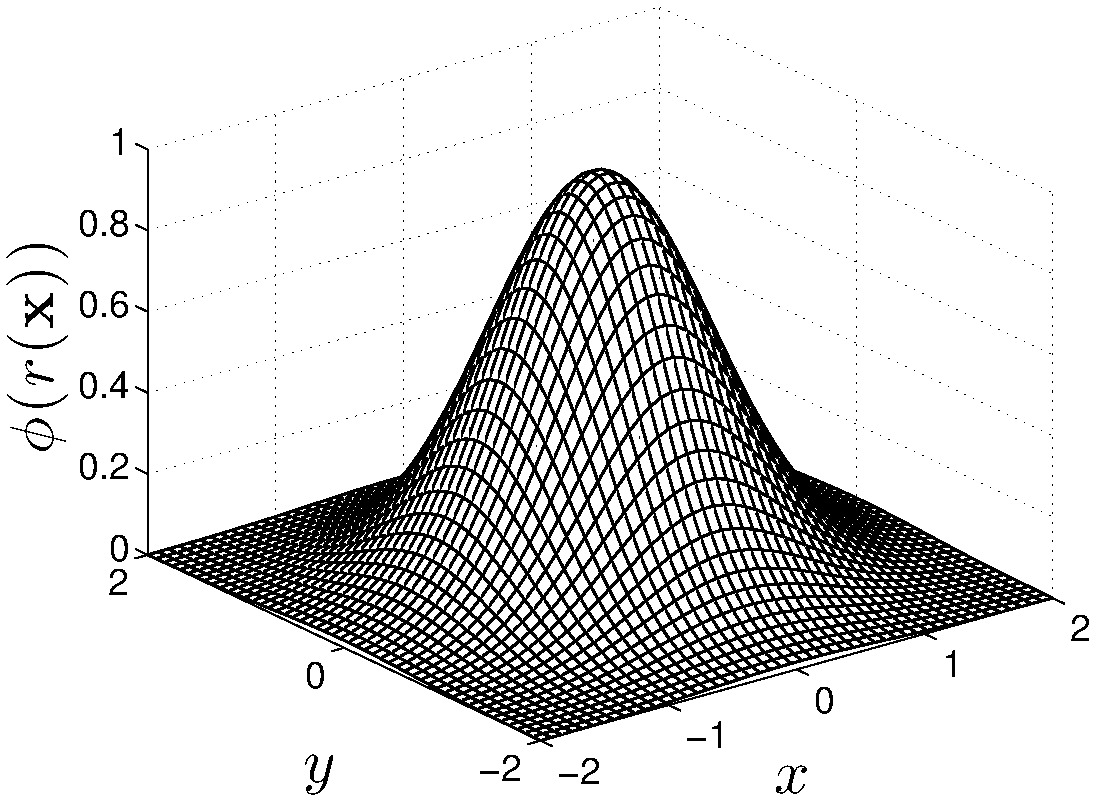
\includegraphics[width=1.0\textwidth]{../figures/paper1/figures/ga_rbf2d-eps-converted-to.pdf} 
		\caption{Gaussian}
	\end{subfigure}
	\begin{subfigure}[b]{0.25\textwidth}
	\centering
		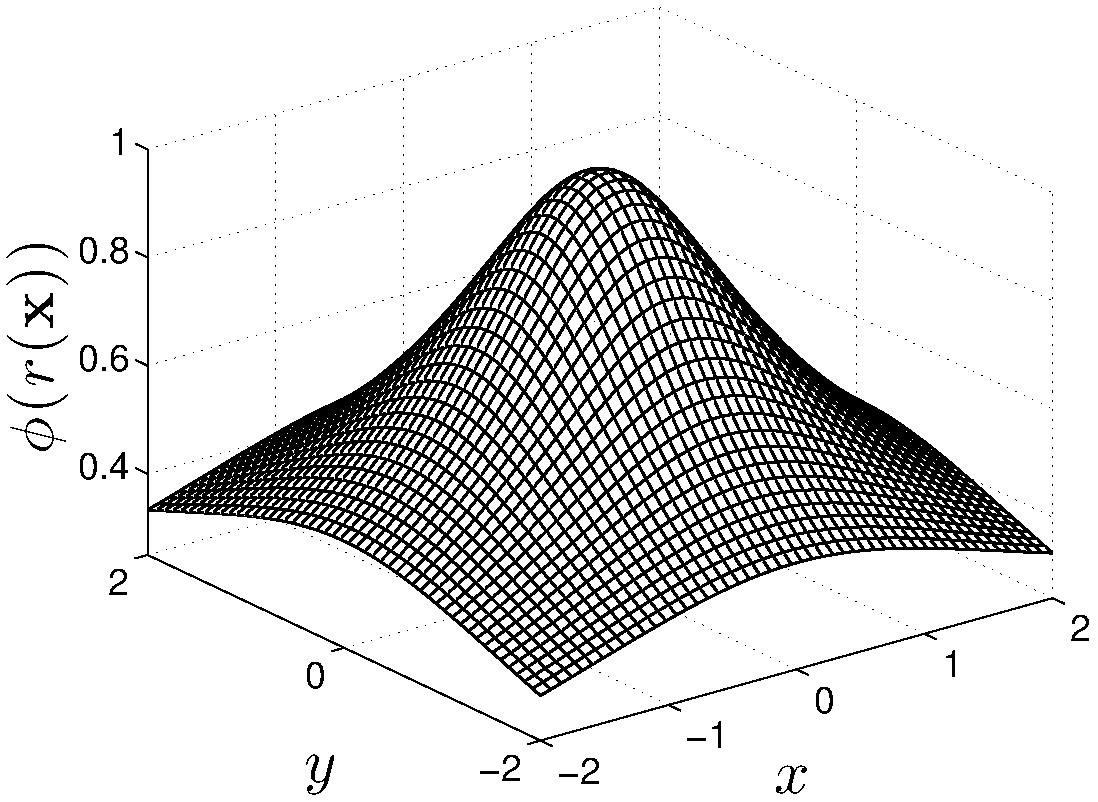
\includegraphics[width=1.0\textwidth]{../figures/paper1/figures/imq_rbf2d-eps-converted-to.pdf}
		\caption{Inverse Multiquadric}
	\end{subfigure}
	\begin{subfigure}[b]{0.25\textwidth}
	\centering
		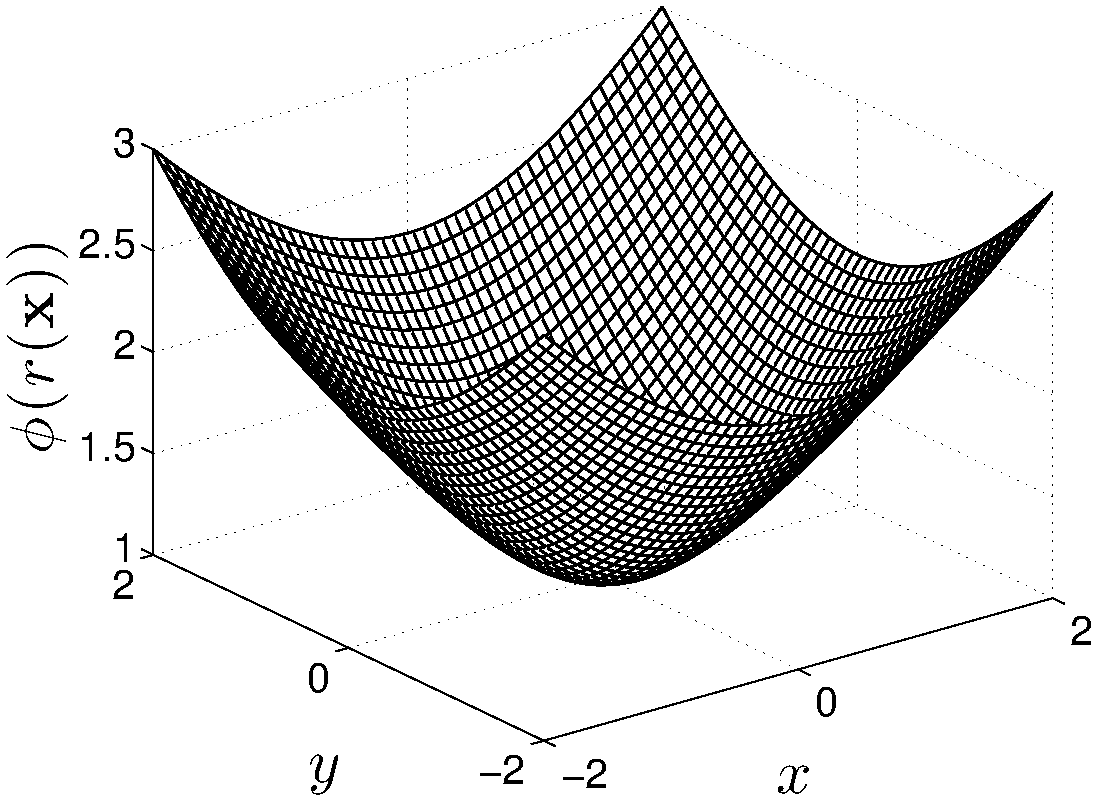
\includegraphics[width=1.0\textwidth]{../figures/paper1/figures/mq_rbf2d-eps-converted-to.pdf} 
		\caption{Multiquadric}
	\end{subfigure} 
    \caption{Commonly Used Radial Basis Functions (RBFs).}
    \label{fig:rbfs}
\end{figure}

At the core of all RBF-based PDE methods lies the fundamental problem of approximation/interpolation. Some methods (e.g., global- and compact-RBF methods) apply RBFs to approximate derivatives directly. Others (e.g., RBF-FD) leverage the basis functions to compute stencil weights, which in turn are used in generalized finite-difference approximations of derivatives. 

As ``meshless" methods, RBF methods excel at solving problems that require geometric flexibility with scattered node layouts in $d$-dimensional space. They naturally extend into higher dimensions with minimal increase in programming complexity \cite{FlyerWright07,WrightFlyerYuen10}. In addition to competitive accuracy and convergence compared with other state-of-the-art methods \cite{FlyerWright07, FlyerWright09, FlyerLehto10, WrightFlyerYuen10, FlyerFornberg11}, RBF methods boast stability for large time steps. Not all RBF methods are truly meshless. Most of them operate the same given an input set of nodes, whether or not the input includes an underlying mesh. However, some methods connect all nodes to all others (to be meshless), while methods like RBF-FD rely on stencils to connect points within small neighborhoods of one another. The generated stencils limit the scope of influence for nodes and complexity of the method, but also simulate a mesh. 

%Most literature surrounding RBF solutions for PDEs apply the concept of collocation (see Chapter~\ref{chap:background}). Recent trends in the community appear to have shifted, and RBF-FD seems to be top of the list. 


%RBF-FD is a hybrid of RBF scattered data interpolation and classical Finite Difference (FD). It shares many of the benefits from other RBF methods, like functionality on scattered node layouts in any dimension and high-order accurate solutions. Likewise, benefits akin to classical FD such as compact stencils for derivative approximation, and low computational complexity.

%Classical FD derivatives are expressed at a single node (center) as a weighted combination/difference of solution values from a small neighborhood (i.e., a stencil) around the center. Common approximations such as upwind differencing, center differencing, and other higher order approximations are of this form. 
%In similar fashion, RBF-FD combines solutions values based on stencils, but it does so in a more generalized sense than standard FD. For example, classical FD is typically restricted to regular meshes and often symmetric stencils in practice with the same set of weights for each stencil. Weights can be derived from polynomial expansion and obtained in 1D by solving a Vandermonde interpolation matrix \cite{FornbergLehto11}. Higher dimension FD stencils are composed from combinations of 1D formulas applied to each dimension. This implies restrictions on the shape/layout of stencils. In contrast to this, RBF-FD is designed for stencils with irregular node placement and can easily provide a unique set of weights for each stencil with no restrictions on stencil shape. 

%TODO:  \cite{Wright2004, Wright2003, WrightFornberg06, Chandhini2007}. 
To track the history of RBF methods, one must rewind to 1971 and R.L. Hardy's seminal research on interpolation with multi-quadric basis functions \cite{Hardy1971}. The transition from interpolation to RBF PDE methods dates back to 1990 \cite{Kansa1990a,Kansa1990b}. 
The RBF-FD method was first introduced in concept in 2000 \cite{Tolstykh2000}, but it took another few years for the method to really get a start (\cite{Shu2003}, \cite{Tolstykh2003a}, \cite{Wright2003} and \cite{Cecil2004}). Now a little over a decade old, the method is finally showing signs that it has the critical-mass following necessary for use in large-scale scientific models. At the onset of this work, most of the literature considered RBF-FD for problem sizes up to a few thousand nodes; at most into tens of thousands of nodes. Similar to most RBF methods, RBF-FD is predominantly implemented within small-scale, serial computing environments. The RBF community at-large continues to depend on MATLAB for investigation and extension development.

The goal of this dissertation is to scale RBF-FD solutions on high resolution meshes across high performance clusters, and to lead the way for its adoption within HPC and supercomputing circles. As part of this push to HPC, leveraging \emph{Graphics Processing Units (GPUs)} for computation is considered critical. GPUs, introduced in Chapter~\ref{chap:gpu_rbffd}, are many-core accelerators capable of general purpose, embarrassingly parallel computations. Accelerators represent the latest trend in HPC, where compute nodes are commonly supplemented by one or more accessory boards for offloading compute intensive tasks. Our effort leads the way for RBF-FD applicationss in an age when compute nodes with attached accelerator boards are considered key to breaching the exa-scale computing barrier \cite{GPUandExascale2011}. 

Parallelization of RBF-FD is achieved at two levels. On the first level, the
physical domain of the problem is partitioned
into overlapping subdomains, each handled by different MPI processes. All processes
operate independently to compute/load RBF-FD stencil weights, run diagnostic
tests and perform other initialization tasks. A process only computes weights
corresponding to stencils centered in the interior of its partition. After
initialization, processes work together to concurrently solve the PDE. Communication
barriers ensure that processes execute in lockstep and maintain consistent
solution values across the domain.  

The second level of
parallelization offloads tasks to the GPU at each iteration of the PDE solver. The bulk of computation in RBF-FD relies on a \emph{Sparse Matrix-Vector multiply (SpMV)} to evaluate derivatives. When mapped to the GPU, the SpMV operation is broken into two parts in order to overlap communication and computation, and amortize the cost of data transfer across multiple levels of hardware (see Chapter~\ref{chap:multigpu_rbffd}). 
% Although the stencil weight calculation is also data-parallel, we assume that in this context that the weights are precomputed and loaded once from disk during the initialization phase. 

%Additional key challenges lie in the choice of grid, the choice of stencil, and stability of scalable solutions. 
%To demonstrate Chapter~\ref{chap:applied_rbffd} verifies 


%
%Even today, RBFs are still up-and-coming in the scientific world with many avenues of research left to consider. Global formulations are understood to have spectral convergence properties, high accuracy and other benefits like adaptivity and ease of implementation over meshed methods \cite{Fasshauer:2007}. However, little is known about the behavior of local and RBF-FD methods. Open questions include (but are in no way limited to): a) ideal node placement to eliminate singularities; b) data-structures for stencil storage and evaluation; c) problem sizes larger than a few thousand nodes; and d) parallel implementations across new heterogeneous multi- and many-core architectures. In response to this, our group, in collaboration with researchers assembled from a national lab and four universities (see Chapter~\ref{chap:funding}), has been granted funds by the National Science Foundation to collaboratively:
%
%\begin{quote}
%\emph{``Bring RBFs to the forefront of multi-scale geophysical modeling by developing fast, efficient, and parallelizable RBF algorithms in arbitrary geometries, with performance enhanced by hardware accelerators, such as graphic processing units (GPUs)."} \cite{RBF_proposal:2009}
%\end{quote}
%
%



The layout of this document is as follows. This chapter continues with a survey of work related to parallelizing RBF-FD, targeting the GPU, and spanning a multi-GPU cluster. Chapter~\ref{chap:background} provides a historical survey of RBF methods as a backdrop to present RBF-FD in Chapter~\ref{chap:rbffd_method}. Chapter~\ref{chap:stencils} introduces a new algorithm for generating RBF-FD stencils as a faster alternative to the RBF community favorite, $k$-D Tree. In Chapter~\ref{chap:distributed_rbffd}, the first scalable implementation of RBF-FD to span one thousand processors is described in detail. Chapter~\ref{chap:gpu_rbffd} continues with the challenge of offloading computation to GPUs, and Chapter~\ref{chap:multigpu_rbffd} expands the discussion to RBF-FD on a multi-GPU cluster. In Chapter~\ref{chap:applications} the parallel RBF-FD implementation is applied and verified on the solutions of both explicit and implicit geophysical PDEs. Finally, Chapter~\ref{chap:conclusions} concludes with a summary of novel contributions, results and a discussion on future directions.

\section{On Parallel/Distributed RBF-FD} 

%TODO: why implement independent of PETSc, Deal.II, Trilinos, etc. 

%\authnote{Related work for start of Parallel/GPU chapter}
Parallel implementations of RBF methods rely on \emph{domain decomposition}. Depending on the implementation, domain decomposition not only accelerates solution procedures, but can decrease the ill-conditioning that plague all global RBF methods (\cite{Divo2007}). The ill-conditioning is reduced if each domain is treated as a separate RBF domain, and the boundary update is treated separately. Domain decomposition methods for RBFs were introduced by Beatson et al. \cite{Beatson2000}. Their work provided a solution to solve problem sizes into the millions of nodes.

This work leverages a domain decomposition, but not for the purpose of conditioning. Instead subdomains are distributed across multiple compute nodes and scaling RBF-FD across more than a thousand CPU cores of an HPC cluster. Add to this a twist to incorporate a novel implementation on the GPU with overlapping communication and computation. This combination is unmatched in related work. However, RBF methods do have a bit of history of parallel implementations. 

In 2007, Divo and Kassab \cite{Divo2007} used a domain decomposition method with artificial 
subdomain boundaries for their implementation of a local collocation method \cite{Divo2007}. 
The subdomains are processed independently, with derivative values 
at artificial boundary points averaged to maintain global consistency of physical values. Their implementation 
was designed for a 36 node cluster, but benchmarks and scalability tests are not provided.

% Divo: it seems almost unnecessary to use domain decomposition if they have the local method.
% I suppose the domain decomposition is necessary for averaging physical values more than RBF collocation.
However, research on the parallelization of RBF algorithms to solve PDEs on multiple CPU/GPU architectures is essentially non-existent. We have found three studies that have addressed this topic, none of which implement RBF-FD but rather take the avenue of domain decomposition for global RBFs (similar to a spectral element approach). In \cite{Divo2007}, Divo and Kassab introduce subdomains with artificial boundaries that are processed independently. Their implementation was designed for a 36 node cluster, but benchmarks and scalability tests are not provided. Kosec and \v{S}arler \cite{Kosec2008} parallelize coupled heat transfer and fluid flow models using OpenMP on a single workstation with one dual-core processor. They achieved a speedup factor of 1.85x over serial execution, although there were
no results from scaling tests. Yokota, Barba and Knepley \cite{Yokota2010} apply a restrictive additive Schwarz domain decomposition to parallelize global RBF interpolation of more then 50 million nodes on 1024 CPU processors.

Kosec and \v{S}arler \cite{Kosec2008} have the only known (to our knowledge) OpenMP implementation for RBFs. The authors parallelize coupled heat transfer 
and fluid flow problems on a single workstation. 
The application involves the local RBF collocation method, explicit time-stepping and Neumann boundary conditions. A speedup 
factor of 1.85x over serial execution was achieved by executing on two CPU cores; no further 
results from scaling tests were provided. 

Stevens et al. \cite{Stevens2009a} mention a parallel implementation under development, but no document is available at this time. 

Perhaps the most competitive parallel implementation of RBFs is the PetRBF branch of PETSc \cite{Yokota2010}. The authors of PetRBF have implemented a highly scalable, efficient RBF interpolation method based on compact RBFs (i.e., they operate on sparse matrices). The authors demonstrate efficient weak scaling of PetRBF across 1024 processes on a Blue Gene/L, and strong scaling up to 128 processes on the same hardware. On the Blue Gene/L, PetRBF is demonstrated to achieve an impressive 74\% parallel weak scaling efficiency on 1024 processes (operating on over 50 million points), and 84\% strong scaling efficiency for 128 processes. Strong scaling was also tested on a Cray XT4, where strong scaling tops out at 36\% for 128 processes, a respectable number---and similar to observed results for our own code on for the same number of processes (see Chapter~\ref{chap:distributed_rbffd}).  


%Within the scope of this paper we detail our method for spanning RBF-FD across multiple CPU/GPU processors and emphasize numerical validation of the implementation rather than optimization strategies. We will consider optimization in future work. The calculations are performed on Keeneland, a high performance computing installation supported by the National Science Foundation and located at Oak Ridge National Lab. Keeneland currently has 240 CPUs accompanied by 360 NVidia Fermi class GPUs with at least double that number expected by the end of 2012 \cite{Vetter2011}.



\section{On GPU RBF Methods (Incomplete)}

With regard to the latter, there is some research on leveraging RBFs on GPUs in the fields of visualization \cite{Cuntz2007,Weiler2005},  surface reconstruction \cite{Corrigan2005,Carr2003}, and neural networks \cite{Brandstetter2008}.

 %Originally GPUs were designed as parallel rasterizing units. They had limited logic control in contrast to the serial CPUs and their advanced branching and looping logic. 
%
%Gradually new and complex logic was added to the GPU to produce the shader languages that allowed developers to customize specific parts of the rendering pipeline. This allowed scientific problems such as the diffusion equation to be solved in process of rendering \cite{Harris2005}. In other words, the GPU was tricked into computing.
%
%The year 2006 brought the modern age of GPU computing with the introduction of CUDA from NVidia. The high level language allowed scientists to leverage the GPU as a parallel accelerator without all of the overhead of setting up graphics contexts and tricking the hardware into computing. Memory management is still the developer's responsibility, but compiler transforms generic C/Fortran code to GPU instruction set. 
%
%Scientific Computing has seen a widespread adoption of GPGPU because of the goal to get to ``exa-scale'' computing, which may only be possible in the near future with the help of GPU accelerators \cite{GPUandExascale2011}. 
%
%NVidia is not the only company involved in many core parallel accelerators. Other groups like AMD and Intel have been increasing the number of cores as well. The end effect is a hybridization where CPUs look similar to GPUs and vice-versa. 
%
%Until 2009, the hardware distinction required that developers target parallelism on CPUs and GPUs using different languages. Then the OpenCL standard was drafted and implemented. OpenCL is a parallel language that strives to provide functional portability rather than performance. 
%
%We focus on the OpenCL language within this dissertation with confidence that hardware will change frequently. In fact, every 18 months \cite{CudaGuide2011} shows a new release of GPU hardware, many-core CPU hardware and extensions to parallel languages. But if hardware is constantly changing, then one must focus on a high level implementation that allows portability across hardware. Enter the Open Compute Language (OpenCL) in 2009. OpenCL is standards based a to carry our implementations into the future regardless of what hardware and which company survive. 


Related work on RBFs and GPUs is sparse. In 2009, Schmidt et al. \cite{Schmidt2009a, Schmidt2009b} implemented a global RBF method for Tsunami simulation on the GPU using the AccelerEyes Jacket \cite{JacketGuide2009} add-on for MATLAB. Jacket provides a MATLAB interface to data structures and routines that internally call to the NVidia CUDA API. Their model was based on a single large dense matrix solve, and with the help of Jacket the authors were able to achieve approximately 7x speedup over the standard MATLAB solution on the then current generation of the MacBook Pro laptop. The authors compared the laptop CPU (processor details not specified) to the built-in NVidia GeForce 8600M GT GPU. Schmidt et al.'s implementation was the first contribution to the RBF community to leverage accelerators. The results were significant and promising, but no further contributions were made on the topic. 

While both Schmidt et al.'s method and the method presented here are based on RBFs, the two problems are only distantly related when it comes to implementation on the GPU. Dense matrix operations have a high computational complexity, are considered ideal (or near to) by linear algebra libraries like BLAS \cite{BLAS} and LAPACK \cite{Lapack1999}, and were demonstrated to fit well on GPUs from the onset of General Purpose GPU (GPGPU) Computing. In fact, NVidia included CUBLAS \cite{CudaToolkitDoc} (a GPU based BLAS library for their hardware) with their initial public release of the game-changing CUDA development kit in 2006. In stark contrast to this, sparse matrix operations have minimal computational complexity and are less than ideal for the GPU.


Earlier this year (2013), Cuomo et al. \cite{Cuomo2013} implemented RBF-interpolation on the GPU for surface reconstruction. Their implementation utilizes PetRBF \cite{Yokota2010}, and new built-in extensions that allow GPU access within PETSc. PETSc internally wraps the CUSP project \cite{Cusp2012} for sparse matrix algebra on the GPU. With the help of these libraries, Cuomo et al. solve and apply sparse interpolation systems on the GPU for up to three million nodes on an NVidia Fermi C1060 GPU (4GB). They compare results to a single core CPU implementation on an Intel i7-940 CPU and demonstrate that the GPU accelerate their solutions between 6x and 25x. Unfortunately, the authors do not show evidence of scaling the interpolation across multiple GPUs; so while evidence exists that PetRBF now has full GPU support, it remains to be seen how well the code can scale in GPU mode. 
 
\section{On Multi-GPU Methods}
 
Multi-GPU Jacobi iteration for Navier stokes flow in cavity \url{http://scholarworks.boisestate.edu/cgi/viewcontent.cgi?article=1003&context=mecheng_facpubs}

Thibault et al. have multiple works on Multi-GPU and overlapping comm and comp. 

The latest version of PETSc includes GPU support. PETSc is a widely-used library for distributed sparse and dense matrix algebra. 

\section{Major Contributions}

Within this thesis readers should expect to find the following major contributions to the communities surrounding RBF methods, GPGPU, and HPC: 
\begin{itemize} 
\item The first implementation of RBF-FD on GPUs, with one and many GPU environments considered. 
\begin{itemize} 
\item Multiple GPU kernels are tested, including custom OpenCL kernels for RK4 time-stepping and 
\end{itemize} 
\item The first implementation of RBF-FD on multiple CPUs through the use of domain decomposition
\item The first application of the Fixed-Grid neighbor query algorithm to generate stencils for RBF-FD. 
\end{itemize}



\ifstandalone
%Bei direkter Übersetzung sollte gleich noch das Literaturverzeichnis rein.
\bibliographystyle{plain}
\bibliography{merged_references}
\end{document}
\else
\expandafter\endinput
\fi


\chapter{Review}
\begin{itemize} 
	\item Review of the Literature (don’t make the mistake of reviewing after rather than before data collection in qualitative studies)
	\item The more references the better
	\item All relevant, reliable, and recent studies be included
	\item Organization is critical 
	\item Compare, contrast, and evaluate previous studies
\end{itemize}

\chapter{Research Methodology}
\begin{itemize} 
	\item Research Perspective: type of methodology and why it is the best way to answer your research question
	\item Context and Access: where, when, and how you will find par(cipants 
 	\item Instrumentation: include copy in appendix or in text if using survey or interview questions
 	\item Procedure: be specific so a reader could imitate your study 
 	\item Data Analysis: again, specific down to the computer program used for statistics
 	\item Qualitative methods
 	\item Data Sources
 	\item Data Collection
 	\item Data Analysis
 	\item Verification
 	\item Ethical Considerations
\end{itemize} 

\chapter{Findings}
\begin{itemize} 
	\item Research Findings (Will be regularly updated)
	\item Presentation of Data (Graphs, charts, tables, etc)
	\item Timings, Convergence Rates, etc.
\end{itemize} 

\chapter{Summary}
\begin{itemize} 
\item Summary (what should readers find in document)
\item Conclusions (what are the improvements made, what algorithms are demonstrated effective?)
\item Discussion
\item Suggestions for future research
\end{itemize} 
%\makeatletter
\@ifundefined{standalonetrue}{\newif\ifstandalone}{}
\@ifundefined{section}{\standalonetrue}{\standalonefalse}
\makeatother
\ifstandalone
\documentclass[11pt]{report}
\usepackage{textcase}
%\usepackage{hyperref}
%\hypersetup{breaklinks=true}


% Added packages
\usepackage[usenames]{color}
\usepackage{amsfonts, amsmath, amssymb, graphics}

% NOTE: bibentry MUST appear before the hyperref or build will fail
\usepackage{bibentry}
\nobibliography*
\usepackage[square,sort,comma,numbers]{natbib}
  
\usepackage{float}
\usepackage[
	hidelinks,%
    %hyperindex=true,		% Make numbers of index links as well
   	backref=page, 		% Provide page listing where refs occur in the bibliography
	%breaklinks=true,
    %colorlinks,%
    %citecolor=green,%
    %filecolor=blue,%
    %linkcolor=red,%
    %urlcolor=red, 
]{hyperref}

\usepackage{dsfont}
%%%% USEPACKAGES for MACROS %%%%%
\usepackage{algpseudocode}
\usepackage[chapter]{algorithm}
%\usepackage{caption}
\usepackage{subcaption}
\usepackage{url}

\usepackage{array}
\usepackage{arydshln}
\usepackage{multirow}
\usepackage{multicol}
%\usepackage[section]{placeins}

\usepackage[usenames,dvipsnames]{color}
%\usepackage[english]{babel}
\usepackage{tabularx}
\usepackage{soul}
\usepackage{xparse}
\usepackage{listings}
%\usepackage[normalem]{ulem}



%%%%%%%%%%%%%%%
% Show a list of items "todo" or "done" 
% USAGE: 
% \begin{todolist} 
% 	\todo Something not finished
% 	\done Something finished
% \end{todolist} 
\newenvironment{todolist}{%
  \begin{list}{}{}% whatever you want the list to be
  \let\olditem\item
  \renewcommand\item{\olditem \textcolor{red}{(TODO)}: }
  \newcommand\todo{\olditem \textcolor{red}{(TODO)}: }
   \newcommand\done{\olditem \textcolor{ForestGreen}{(DONE)}: }
}{%
  \end{list}
} 
%%%%%%%%%%%%%%%

%%%%%%%%%%%%%%%
% Show a Author's Note
% USAGE: 
% \incomplete[Optional footnote message to further clarify note]{The text which is currently not finished}
\DeclareDocumentCommand \incomplete{ o m }
{%
\IfNoValueTF {#1}
{\textcolor{red}{Incomplete: \ul{#2}}} 
{\textcolor{red}{Incomplete: \ul{#2}}\footnote{Comment: #1}}%
}
%%%%%%%%%%%%%%%



%%%%%%%%%%%%%%%
% Show a Author's Note
% USAGE: 
% \authnote[Optional footnote message to further clarify note]{The note to your readers}
\DeclareDocumentCommand \authnote { o m }
{%
\IfNoValueTF {#1}
{\textcolor{blue}{Author's Note: \ul{#2}}} 
{\textcolor{blue}{Author's Note: \ul{#2}}\footnote{Comment: #1}}%
}
%%%%%%%%%%%%%%%



%%%%%%%%%%%%%%%
% Strike out text that doesn't belong in the paper
% USAGE: 
% \strike[Optional footnote to state why it doesn't belong]{Text to strike out}
\DeclareDocumentCommand \strike { o m }
{%
\setstcolor{Red}
\IfNoValueTF {#1}
{\textcolor{Gray}{\st{#2}}} 
{\textcolor{Gray}{\st{#2}}\footnote{Comment: #1}}%
}
%%%%%%%%%%%%%%%

\definecolor{light-gray}{gray}{0.95}

\newcommand{\cbox}[3]{
\ \\
\fcolorbox{#1}{#2}{
\parbox{\textwidth}{
#3
}
}
}

% Setup an environment similar to verbatim but which will highlight any bash commands we have
\lstnewenvironment{unixcmds}[0]
{
%\lstset{language=bash,frame=shadowbox,rulesepcolor=\color{blue}}
\lstset{ %
language=sh,		% Language
basicstyle=\ttfamily,
backgroundcolor=\color{light-gray}, 
rulecolor=\color{blue},
%frame=tb, 
columns=fullflexible,
%framexrightmargin=-.2\textwidth,
linewidth=0.8\textwidth,
breaklines=true,
%prebreak=/, 
  prebreak = \raisebox{0ex}[0ex][0ex]{\ensuremath{\hookleftarrow}},
%basicstyle=\footnotesize,       % the size of the fonts that are used for the code
%numbers=left,                   % where to put the line-numbers
%numberstyle=\footnotesize,      % the size of the fonts that are used for the line-numbers
%stepnumber=2,                   % the step between two line-numbers. If it's 1 each line 
                                % will be numbered
%numbersep=5pt,                  % how far the line-numbers are from the code
showspaces=false,               % show spaces adding particular underscores
showstringspaces=false,         % underline spaces within strings
showtabs=false,                 % show tabs within strings adding particular underscores
frame=single,	                % adds a frame around the code
tabsize=2,	                % sets default tabsize to 2 spaces
captionpos=b,                   % sets the caption-position to bottom
breakatwhitespace=false,        % sets if automatic breaks should only happen at whitespace
}
} { }

% Setup an environment similar to verbatim but which will highlight any bash commands we have
\lstnewenvironment{cppcode}[1]
{
%\lstset{language=bash,frame=shadowbox,rulesepcolor=\color{blue}}
\lstset{ %
	backgroundcolor=\color{light-gray}, 
	rulecolor=\color[rgb]{0.133,0.545,0.133},
	tabsize=4,
	language=[GNU]C++,
%	basicstyle=\ttfamily,
        basicstyle=\scriptsize,
        upquote=true,
        aboveskip={1.5\baselineskip},
        columns=fullflexible,
        %framexrightmargin=-.1\textwidth,
       %framexleftmargin=6mm,
        showstringspaces=false,
        extendedchars=true,
        breaklines=true,
        prebreak = \raisebox{0ex}[0ex][0ex]{\ensuremath{\hookleftarrow}},
        frame=single,
        showtabs=false,
        showspaces=false,
        showstringspaces=false,
        numbers=left,                   % where to put the line-numbers
	numberstyle=\footnotesize,      % the size of the fonts that are used for the line-numbers
	stepnumber=4,                   % the step between two line-numbers. If it's 1 each line 
                                % will be numbered
	firstnumber=#1,
         numbersep=5pt,                  % how far the line-numbers are from the code
        identifierstyle=\ttfamily,
        keywordstyle=\color[rgb]{0,0,1},
        commentstyle=\color[rgb]{0.133,0.545,0.133},
        stringstyle=\color[rgb]{0.627,0.126,0.941},
}
} { }

% Setup an environment similar to verbatim but which will highlight any bash commands we have
\lstnewenvironment{mcode}[1]
{
\lstset{ %
	backgroundcolor=\color{light-gray}, 
	rulecolor=\color[rgb]{0.133,0.545,0.133},
	tabsize=4,
	language=Matlab,
%	basicstyle=\ttfamily,
        basicstyle=\scriptsize,
        upquote=true,
        aboveskip={1.5\baselineskip},
        columns=fullflexible,
        %framexrightmargin=-.1\textwidth,
       %framexleftmargin=6mm,
        showstringspaces=false,
        extendedchars=true,
        breaklines=true,
        prebreak = \raisebox{0ex}[0ex][0ex]{\ensuremath{\hookleftarrow}},
        frame=single,
        showtabs=false,
        showspaces=false,
        showstringspaces=false,
        numbers=left,                   % where to put the line-numbers
	numberstyle=\footnotesize,      % the size of the fonts that are used for the line-numbers
	stepnumber=4,                   % the step between two line-numbers. If it's 1 each line 
                                % will be numbered
	firstnumber=#1,
         numbersep=5pt,                  % how far the line-numbers are from the code
        identifierstyle=\ttfamily,
        keywordstyle=\color[rgb]{0,0,1},
        commentstyle=\color[rgb]{0.133,0.545,0.133},
        stringstyle=\color[rgb]{0.627,0.126,0.941},
}
} { }

\newcommand{\inputmcode}[1]{%
\lstset{ %
	backgroundcolor=\color{light-gray},  %
	rulecolor=\color[rgb]{0.133,0.545,0.133}, %
	tabsize=4, %
	language=Matlab, %
%	basicstyle=\ttfamily,
        basicstyle=\scriptsize, %
        %        upquote=true,
        aboveskip={1.5\baselineskip}, %
        columns=fullflexible, %
        %framexrightmargin=-.1\textwidth,
       %framexleftmargin=6mm,
        showstringspaces=false, %
        extendedchars=true, %
        breaklines=true, %
        prebreak = \raisebox{0ex}[0ex][0ex]{\ensuremath{\hookleftarrow}}, %
        frame=single, %
        showtabs=false, %
        showspaces=false, %
        showstringspaces=false,%
        numbers=left,                   % where to put the line-numbers
	numberstyle=\footnotesize,      % the size of the fonts that are used for the line-numbers
	stepnumber=4,                   % the step between two line-numbers. If it's 1 each line 
                                % will be numbered
         numbersep=5pt,                  % how far the line-numbers are from the code
        identifierstyle=\ttfamily, %
        keywordstyle=\color[rgb]{0,0,1}, %
        commentstyle=\color[rgb]{0.133,0.545,0.133}, %
        stringstyle=\color[rgb]{0.627,0.126,0.941} %
}
\lstinputlisting{#1}%
}

%\lstset{ %
%	backgroundcolor=\color{light-gray}, 
%	rulecolor=\color[rgb]{0.133,0.545,0.133},
%	tabsize=4,
%	language=Matlab,
%%	basicstyle=\ttfamily,
%        basicstyle=\scriptsize,
%        upquote=true,
%        aboveskip={1.5\baselineskip},
%        columns=fullflexible,
%        %framexrightmargin=-.1\textwidth,
%       %framexleftmargin=6mm,
%        showstringspaces=false,
%        extendedchars=true,
%        breaklines=true,
%        prebreak = \raisebox{0ex}[0ex][0ex]{\ensuremath{\hookleftarrow}},
%        frame=single,
%        showtabs=false,
%        showspaces=false,
%        showstringspaces=false,
%        numbers=left,                   % where to put the line-numbers
%	numberstyle=\footnotesize,      % the size of the fonts that are used for the line-numbers
%	stepnumber=4,                   % the step between two line-numbers. If it's 1 each line 
%                                % will be numbered
%	firstnumber=#1,
%         numbersep=5pt,                  % how far the line-numbers are from the code
%        identifierstyle=\ttfamily,
%        keywordstyle=\color[rgb]{0,0,1},
%        commentstyle=\color[rgb]{0.133,0.545,0.133},
%        stringstyle=\color[rgb]{0.627,0.126,0.941},
%}


\newcommand{\Laplacian}[1]{\nabla^2 #1}

% set of all nodes received and contained on GPU
\newcommand{\setAllNodes}[0]{\mathcal{G}}
% set of stencil centers on GPU
\newcommand{\setCenters}[0]{\mathcal{Q}}
% set of stencil centers with nodes in \setDepend
\newcommand{\setBoundary}[0]{\mathcal{B}}
% set of nodes received by other GPUs
\newcommand{\setDepend}[0]{\mathcal{R}}
% set of nodes sent to other GPUs
\newcommand{\setProvide}[0]{\mathcal{O}}


\newcommand{\toprule}[0]{\hline}
\newcommand{\midrule}[0]{\hline\hline}
\newcommand{\bottomrule}[0]{\hline}

\newcolumntype{C}{>{\centering\arraybackslash}b{1in}}
\newcolumntype{L}{>{\flushleft\arraybackslash}b{1.5in}}
\newcolumntype{R}{>{\flushright\arraybackslash}b{1.5in}}
\newcolumntype{D}{>{\flushright\arraybackslash}b{2.0in}}
\newcolumntype{E}{>{\flushright\arraybackslash}b{1.0in}}

\DeclareSymbolFont{AMSb}{U}{msb}{m}{n}
\DeclareMathSymbol{\N}{\mathbin}{AMSb}{"4E}
\DeclareMathSymbol{\Z}{\mathbin}{AMSb}{"5A}
\DeclareMathSymbol{\R}{\mathbin}{AMSb}{"52}
\DeclareMathSymbol{\Q}{\mathbin}{AMSb}{"51}
\DeclareMathSymbol{\PP}{\mathbin}{AMSb}{"50}
\DeclareMathSymbol{\I}{\mathbin}{AMSb}{"49}
%\DeclareMathSymbol{\C}{\mathbin}{AMSb}{"43}

%%%%%% VECTOR NORM: %%%%%%%
\newcommand{\vectornorm}[1]{\left|\left|#1\right|\right|}
\newcommand{\vnorm}[1]{\left|\left|#1\right|\right|}
\newcommand{\by}[0]{\times}
\newcommand{\vect}[1]{\mathbf{#1}}
%\newcommand{\mat}[1]{\mathbf{#1}} 

%\renewcommand{\vec}[1]{ \textbf{#1} }
%%%%%%%%%%%%%%%%%%%%%%

%%%%%%% THM, COR, DEF %%%%%%%
%\newtheorem{theorem}{Theorem}[section]
%\newtheorem{lemma}[theorem]{Lemma}
%\newtheorem{proposition}[theorem]{Proposition}
%\newtheorem{corollary}[theorem]{Corollary}
%\newenvironment{proof}[1][Proof]{\begin{trivlist}
%\item[\hskip \labelsep {\bfseries #1}]}{\end{trivlist}}
%\newenvironment{definition}[1][Definition]{\begin{trivlist}
%\item[\hskip \labelsep {\bfseries #1}]}{\end{trivlist}}
%\newenvironment{example}[1][Example]{\begin{trivlist}
%\item[\hskip \labelsep {\bfseries #1}]}{\end{trivlist}}
%\newenvironment{remark}[1][Remark]{\begin{trivlist}
%\item[\hskip \labelsep {\bfseries #1}]}{\end{trivlist}}
%\newcommand{\qed}{\nobreak \ifvmode \relax \else
%      \ifdim\lastskip<1.5em \hskip-\lastskip
%      \hskip1.5em plus0em minus0.5em \fi \nobreak
%      \vrule height0.75em width0.5em depth0.25em\fi}
%%%%%%%%%%%%%%%%%%%%%%

%
%\usepackage[algochapter]{algorithm2e}
%\usepackage[usenames]{color}
% colors to show the corrections
\newcommand{\red}[1]{\textbf{\textcolor{red}{#1}}}
\newcommand{\blue}[1]{\textbf{\textcolor{blue}{#1}}}
\newcommand{\cyan}[1]{\textbf{\textcolor{cyan}{#1}}}
\newcommand{\green}[1]{\textbf{\textcolor{green}{#1}}}
\newcommand{\magenta}[1]{\textbf{\textcolor{magenta}{#1}}}
\newcommand{\orange}[1]{\textbf{\textcolor{orange}{#1}}}
%%%%%%%%%% DK DK
% comments between authors
\newcommand{\toall}[1]{\textbf{\green{@@@ All: #1 @@@}}}
\newcommand{\toevan}[1]{\textbf{\red{*** Evan: #1 ***}}}
%\newcommand{\toevan}[1]{}  % USE FOR FINAL VERSION
\newcommand{\toe}[1]{\textbf{\red{*** Evan: #1 ***}}}
\newcommand{\tog}[1]{\textbf{\blue{*** Gordon: #1 ***}}}
%\newcommand{\togordon}[1]{\textbf{\blue{*** Gordon: #1 ***}}}
\renewcommand{\ge}[3]{{\textcolor{blue}{*** \textbf{Gordon:}\strike{#1} #2 ***}}\red{(#3)}}
\renewcommand{\ge}[3]{{\textcolor{blue}{#2}}}
\renewcommand{\ge}[3]{{\textcolor{Red}{#2}}}
\newcommand{\eb}[3]{{\textcolor{Red}{*** \textbf{Evan:}\strike{#1} #2 ***}}\red{(#3)}}
\renewcommand{\eb}[3]{{{\textcolor{Red}{#2}}}}
%\def\ge#1#2#3{}{\textbf{\blue{*** Gordon: #2 ***}}}{(#3)}
\newcommand{\gee}[1]{{\bf{\blue{{\em #1}}}}}
\newcommand{\old}[1]{}
\newcommand{\del}[1]{***#1*** }



% \DeclareMathOperator{\Sample}{Sample}
%\let\vaccent=\v % rename builtin command \v{} to \vaccent{}
%\renewcommand{\vec}[1]{\ensuremath{\mathbf{#1}}} % for vectors
\newcommand{\gv}[1]{\ensuremath{\mbox{\boldmath$ #1 $}}} 
% for vectors of Greek letters
\newcommand{\uv}[1]{\ensuremath{\mathbf{\hat{#1}}}} % for unit vector
\newcommand{\abs}[1]{\left| #1 \right|} % for absolute value
\newcommand{\avg}[1]{\left< #1 \right>} % for average
\let\underdot=\d % rename builtin command \d{} to \underdot{}
\renewcommand{\d}[2]{\frac{d #1}{d #2}} % for derivatives
\newcommand{\dd}[2]{\frac{d^2 #1}{d #2^2}} % for double derivatives
\newcommand{\pd}[2]{\frac{\partial #1}{\partial #2}} 
% for partial derivatives
\newcommand{\pdd}[2]{\frac{\partial^2 #1}{\partial #2^2}} 
\newcommand{\pdda}[3]{\frac{\partial^2 #1}{\partial #2 \partial #3}} 
% for double partial derivatives
\newcommand{\pdc}[3]{\left( \frac{\partial #1}{\partial #2}
 \right)_{#3}} % for thermodynamic partial derivatives
\newcommand{\ket}[1]{\left| #1 \right>} % for Dirac bras
\newcommand{\bra}[1]{\left< #1 \right|} % for Dirac kets
\newcommand{\braket}[2]{\left< #1 \vphantom{#2} \right|
 \left. #2 \vphantom{#1} \right>} % for Dirac brackets
\newcommand{\matrixel}[3]{\left< #1 \vphantom{#2#3} \right|
 #2 \left| #3 \vphantom{#1#2} \right>} % for Dirac matrix elements
\newcommand{\grad}[1]{\gv{\nabla} #1} % for gradient
\let\divsymb=\div % rename builtin command \div to \divsymb
\renewcommand{\div}[1]{\gv{\nabla} \cdot #1} % for divergence
\newcommand{\curl}[1]{\gv{\nabla} \times #1} % for curl
\let\baraccent=\= % rename builtin command \= to \baraccent
\renewcommand{\=}[1]{\stackrel{#1}{=}} % for putting numbers above =
\newcommand{\diffop}[1]{\mathcal{L}#1}
\newcommand{\boundop}[1]{\mathcal{B}#1}
\newcommand{\rvec}[0]{{\bf r}}

\newcommand{\Interior}[0]{\Omega}
\newcommand{\domain}[0]{\Omega}
%\newcommand{\Boundary}[0]{\partial \Omega}
\newcommand{\Boundary}[0]{\Gamma}

\newcommand{\on}[1]{\hskip1.5em \textrm{ on } #1}

\newcommand{\gemm}{\texttt{GEMM}}
\newcommand{\trmm}{\texttt{TRMM}}
\newcommand{\gesvd}{\texttt{GESVD}}
\newcommand{\geqrf}{\texttt{GEQRF}}


\newcommand{\minitab}[2][l]{\begin{tabular}{#1}#2\end{tabular}}
\newcommand{\comm}[1]{\textcolor{red}{\textit{#1}}}

\newcommand{\nfrac}[2]{
\nicefrac{#1}{#2}
%\frac{#1}{#2}
}

\usepackage{xparse}
\usepackage{soul}


%%%%%%%%%%%%%%%
% Show a Author's Note
% USAGE: 
% \incomplete[Optional footnote message to further clarify note]{The text which is currently not finished}
\DeclareDocumentCommand \incomplete{ o m }
{%
\IfNoValueTF {#1}
{\textcolor{red}{Incomplete: \ul{#2}}} 
{\textcolor{red}{Incomplete: \ul{#2}}\footnote{Comment: #1}}%
}
%%%%%%%%%%%%%%%



%%%%%%%%%%%%%%%
% Show a Author's Note
% USAGE: 
% \authnote[Optional footnote message to further clarify note]{The note to your readers}
\DeclareDocumentCommand \authnote { o m }
{%
\IfNoValueTF {#1}
{\textcolor{blue}{Author's Note: \ul{#2}}} 
{\textcolor{blue}{Author's Note: \ul{#2}}\footnote{Comment: #1}}%
}
%%%%%%%%%%%%%%%



%%%%%%%%%%%%%%%
% Strike out text that doesn't belong in the paper
% USAGE: 
% \strike[Optional footnote to state why it doesn't belong]{Text to strike out}
\DeclareDocumentCommand \strike { o m }
{%
\setstcolor{red}
\IfNoValueTF {#1}
{\textcolor{Gray}{\st{#2}}} 
{\textcolor{Gray}{\st{#2}}\footnote{Comment: #1}}%
}
%%%%%%%%%%%%%%%



%
% colors to show the corrections
\newcommand{\red}[1]{\textbf{\textcolor{red}{#1}}}
\newcommand{\blue}[1]{\textbf{\textcolor{blue}{#1}}}
\newcommand{\cyan}[1]{\textbf{\textcolor{cyan}{#1}}}
\newcommand{\green}[1]{\textbf{\textcolor{green}{#1}}}
\newcommand{\magenta}[1]{\textbf{\textcolor{magenta}{#1}}}
\newcommand{\orange}[1]{\textbf{\textcolor{orange}{#1}}}
%%%%%%%%%% DK DK
% comments between authors
\newcommand{\toall}[1]{\textbf{\green{@@@ All: #1 @@@}}}
\newcommand{\toevan}[1]{\textbf{\red{*** Evan: #1 ***}}}
%\newcommand{\toevan}[1]{}  % USE FOR FINAL VERSION
\newcommand{\toe}[1]{\textbf{\red{*** Evan: #1 ***}}}
\newcommand{\tog}[1]{\textbf{\blue{*** Gordon: #1 ***}}}
%\newcommand{\togordon}[1]{\textbf{\blue{*** Gordon: #1 ***}}}
\renewcommand{\ge}[3]{{\textcolor{blue}{*** \textbf{Gordon:}\strike{#1} #2 ***}}\red{(#3)}}
\renewcommand{\ge}[3]{{\textcolor{blue}{#2}}}
\renewcommand{\ge}[3]{{\textcolor{red}{#2}}}
\newcommand{\eb}[3]{{\textcolor{red}{*** \textbf{Evan:}\strike{#1} #2 ***}}\red{(#3)}}
\renewcommand{\eb}[3]{{{\textcolor{red}{#2}}}}
%\def\ge#1#2#3{}{\textbf{\blue{*** Gordon: #2 ***}}}{(#3)}
\newcommand{\gee}[1]{{\bf{\blue{{\em #1}}}}}
\newcommand{\old}[1]{}
\newcommand{\del}[1]{***#1*** }



% Rename  this file          misc_mac.tex
%----------------------------------------------------------------------
%%%%%%%%%%%%%%%%%%%%%%%%%%%%%%%%%%%%%%%%%%%%%%%%%%%%%%%%%%%%%%%%%%%%%%%%%%%%%%%
%
%	Math Symbols   Math Symbols   Math Symbols   Math Symbols   
%
%%%%%%%%%%%%%%%%%%%%%%%%%%%%%%%%%%%%%%%%%%%%%%%%%%%%%%%%%%%%%%%%%%%%%%%%%%%%%%%
\def\pmb#1{\setbox0=\hbox{$#1$}%
	\kern-.025em\copy0\kern-\wd0
	\kern.05em\copy0\kern-\wd0
	\kern-.025em\raise.0433em\box0}
\def\pmbf#1{\pmb#1}
\def\bfg#1{\pmb#1}

% BETTER VALUES FOR AUTOMATIC FIGURE PLACEMENT THAN THOSE PROVIDED BY 
% LATEX DEFAULTS.

\renewcommand{\textfloatsep}{1ex}
\renewcommand{\floatpagefraction}{0.9}
\renewcommand{\intextsep}{1ex}
\renewcommand{\topfraction}{.9}
\renewcommand{\bottomfraction}{.9}
\renewcommand{\textfraction}{.1}

% #1  position of floating figure (h|t|b|p)
% #1  EPS postscript file
% #2  size
% #3  caption

%usage of newfig:
%  \newfig{file.ps}{3in}{Fig1: this is a figure}

\input{epsf}
\def\newfig#1#2#3{
  \begin{figure}[htbp]
  \vspace{1ex}
  \setlength{\epsfxsize}{#2}
  \centerline{\epsfbox{#1}}
  \vspace{-.1in}\caption{\small #3}\break\vspace{.2in}
  \label{#1}
  \end{figure}
}

%usage of newfigtwo: 2 figures, vertically stacked
% \newfig
%	{file1.ps}
%	{file2.ps}
%	{width}
%	{vertical space}
%	{Caption}

\def\newfigtwo#1#2#3#4#5{
  \begin{figure}[htbp]
  \vspace{1ex}
  \setlength{\epsfxsize}{#3}
  \centerline{\epsfbox{#1}}
  \vspace{#4}
  \setlength{\epsfxsize}{#3}
  \centerline{\epsfbox{#2}}
  \vspace{-.1in}\caption{\small #5}\break\vspace{.2in}
  \label{#1}
  \end{figure}
}

\def\newfigh#1#2#3#4{  % add height specification
  \begin{figure}[htbp]
  \vspace{1ex}
  \setlength{\epsfxsize}{#2}
  \setlength{\epsfysize}{#4}
  \centerline{\epsfbox{#1}}
  \vspace{-.1in}\caption{\small #3}\break\vspace{.2in}
  \label{#1}
  \end{figure}
}

\def\herefig#1#2#3{
  \begin{figure}[h]
  \setlength{\epsfxsize}{#2}
  \centerline{\epsfbox{#1}}
  \caption{\small #3}
  \label{#1}
  \end{figure}
}

\def\etal{{{\em et~al.\,\,}}}
\def\note#1{\\ =====#1===== \\}
\def\FBOX#1{\ \\ \fbox{\begin{minipage}{5in}#1\end{minipage}}\\ }
\newcount\sectionno     \sectionno=0
\newcount\eqnum         \eqnum=0
\def\addeqno{\global\advance \eqnum by  1 }
\def\subeqno{\global\advance \eqnum by -1 }
%\def\eqn{\addeqno \eqno \hbox{(\number\sectionno.\number\eqnum)} }

\def\tildetilde#1{\tilde{\tilde{#1}}}
\def\barbar#1{\overbar{\overbar{#1}}}

\def\vsp#1{\vspace{#1 ex}}
\def\fpar{\hspace{\parindent}}
%
%  \pf : 2 arguments: numerator and denominator of partial derivative
%
\def\pf#1#2{{\frac{\partial{#1}}{\partial{#2}}}}
\def\pfs#1#2{{\partial_{#2}{#1}}}
\def\pftwo#1#2{{\frac{\partial^2{#1}}{\partial{#2}^2}}}
\def\pfxx#1#2{{\frac{\partial^2{#1}}{\partial{#2}^2}}}
%\def\pfxy#1#2{{\frac{\partial^2{#1}}{\partial{#2}\partial{#3}}}}
\def\pfn#1#2#3{{\frac{\partial^{#1}{#2}}{\partial{#3}^{#1}}}}
\def\df#1#2{{\frac{d{#1}}{d{#2}}}}
\def\dfn#1#2#3{{\frac{d^{#1}{#2}}{d{#3}^{#1}}}}
\def\Dt#1#2{\frac{D#1}{D#2}}
\def\dt#1#2{\frac{d#1}{d#2}}
\def\bld#1{{\bf #1}}
\def\pfp#1#2#3{\pf{}{#3}{\left(\frac{#1}{#2}\right)}}

\def\norm#1{\|#1\|}

%
% Graphic characters  (\dot already defined by TeX/LateX)
%
\def\dash{\rule[1.5pt]{2mm}{.3mm}\HS{.9mm}}
\def\dott{\rule[1.5pt]{.7mm}{.3mm}\HS{.7mm}}
\def\dashline{\dash\dash\dash}
\def\dotline{\dott\dott\dott\dott\dott\dott}
\def\dashdotline{\dash$\cdot$\HS{.9mm}\dash}
\def\solidline{\rule[2pt]{7mm}{.3mm}}
% 
% overcircle
%
\def\ovcircle#1{\buildrel{\circ}\over{#1}}
%\def\below#1#2{\buildrel{#2}\under{#1}}
%\def\above#1#2{\buildrel{#2}\over{#1}}
%
%  big parenthesis and brackets
%
\def\bigpar#1#2{{\left(\frac{#1}{#2}\right)}}
\def\bigbra#1#2{{\left\[\frac{#1}{#2}\right\]}}

\def\Lp{\left(}
\def\Rp{\right)}
\def\Lb{\left[}
\def\Rb{\right]}
\def\Ln{\left\langle}
\def\Rn{\right\rangle}
\def\Ld{\left.}
\def\Rd{\right.}
\def\Lv{\left|}
\def\Rv{\right|}
\def\Lbr{\left|}
\def\Rbr{\right|}
\def\lng{\langle}
\def\rng{\rangle}
\def\Lc{\left\{}
\def\Rc{\right\}}
%%% %

% Cannot be handled by Lyx
%\def\[{{[}}
%\def\]{{]}}

%
\def\eol{\nonumber \\}
\def\eolnonb{\nonumber\\}
\def\eolnb{\\}
\def\nonb{\nonumber}
\def\be{\begin{equation}}
\def\ee{\end{equation}}
\def\BEQNA{\begin{eqnarray}}
\def\EEQNA{\end{eqnarray}}
\def\eqa{&=&}
\def\beqna{\begin{eqnarray}}
\def\eeqna{\end{eqnarray}}
\def\bverb{\begin{verbatim}}
\def\everb{\end{verbatim}}
\def\VERB#1{\bverb #1 \everb}
\def\btbl{\begin{tabular}}
\def\etbl{\end{tabular}}
\def\bmini{\begin{minipage}[t]{5.5in}}
\def\emini{\end{minipage}}
\def\parray#1#2{\left(\begin{array}{#1}#2\end{array}\right)}
\def\barray#1#2{\left[\begin{array}{#1}#2\end{array}\right]}
\def\carray#1#2{\left\{\begin{array}{#1}#2\end{array}\right.}
\def\darray#1#2{\left|\begin{array}{#1}#2\end{array}\right|}

\def\BEGTABLE#1{\begin{table}[hbt]\vspace{2ex}\begin{center}\bmini\centering\btbl{#1}}
\def\ENDTABLE#1#2{\etbl\caption[#1]{#2}\EMINI\end{center}\vspace{2ex}\end{table}}

\def\bfltbl#1{\begin{table}[hbt]\vspace{2ex}\begin{center}\bmini\centering\btbl{#1}}
\def\efltbl#1#2{\etbl\caption[#1]{#2}\emini\end{center}\vspace{2ex}\end{table}}
\def\mcol{\multicolumn}
%
%  label equations with (#)
%
\def\reff#1{(\ref{#1})}
%
%  macros borrowed from viewgraph package
%

\newenvironment{LETTRS}[3]{\begin{letter}{#1}
\input{origin}\opening{Dear #2:}\input{#3}\closing{Sincerely yours,}\end{letter}}{\clearpage}

\newenvironment{VIEW}[1]{{\BC\Huge\bf #1 \EC}\LARGE\VS{.05in}}{\clearpage}

\def\RM#1{\rm{#1\ }}
\def\BV{\begin{VIEW}}
\def\EV{\end{VIEW}}

\def\NI{\noindent}

\def\VS{\vspace*}
\def\HS{\hspace*}
\def\IT{\item}

\def\BARR{\begin{array}}
\def\EARR{\end{array}}

\def\BPARR{\left(\begin{array}}
\def\EPARR{\end{array}\right)}

\def\BDET{\left|\begin{array}}
\def\EDET{\end{array}\right|}

\def\BDF{\begin{definition}}
\def\EDF{\end{definition}}

\def\BSU{\begin{block}{Summary}}
\def\ESU{\end{block}}

\def\BEX{\begin{example}}
\def\EEX{\end{example}}

\def\BTH{\begin{theorem}}
\def\ETH{\end{theorem}}

\def\BCO{\begin{corollary}}
\def\ECO{\end{corollary}}

\def\BPROOF{\begin{proof}}
\def\EPROOF{\end{proof}}

\def\BLM{\begin{lemma}}
\def\ELM{\end{lemma}}

\def\BEQ{\begin{equation}}
\def\EEQ{\end{equation}}

\def\BEQNNB{$$}
\def\EEQNNB{$$}

\def\BE{\begin{enumerate}}
\def\EE{\end{enumerate}}

\def\BD{\begin{description}}
\def\ED{\end{description}}

\def\BI{\begin{itemize}}
\def\EI{\end{itemize}}

\def\BC{\begin{center}}
\def\EC{\end{center}}

\def\BFIG{\begin{figure}}
\def\EFIG{\end{figure}}

\def\BTABB{\begin{tabbing}}
\def\ETABB{\end{tabbing}}

\def\BMINI{\begin{minipage}}
\def\EMINI{\end{minipage}}

\def\BTABLE{\begin{table}}
\def\ETABLE{\end{table}}

\def\BTABUL{\begin{tabular}}
\def\ETABUL{\end{tabular}}

\def\MCOL{\multicolumn}
\def\UL{\underline}
\def\ULL#1{\UL{\UL{#1}}}

\def\BDOC{\begin{document}}
\def\EDOC{\end{document}}

\def\EM#1{{\em #1\/}}
\def\FN{\footnote}

% Courtesy of Ugo Piomelli

\def\latexfig #1 #2 #3 #4 #5 {\ \vfill
\hfill\hbox to 0.05in{\vbox to #3truein{
         \special{psfile="#1" angle=270 hscale=100 
                  hoffset=#4 voffset=#5 vscale=100} }\hfill}
\hfill\vspace{-0.1in}        }

% #1 is the .ps filename
% #2 is not used in the present version
% #3 is the size of the white space left above the caption (in inches)
% #4 is the horizontal offset from some unknown reference point.
%    It is in 1/72 of an inch and is positive to the right.
% #5 is the vertical offset from some unknown reference point.
%    It is in 1/72 of an inch and is positive upwards.


\newcommand{\mathsym}[1]{{}}
\newcommand{\unicode}[1]{{}}
\newcommand{\ep}{\epsilon}
\newcommand{\vv}{\mathbf{v}}
\newcommand{\vu}{\mathbf{u}}
\newcommand{\vx}{\mathbf{x}}

\newcommand{\Laplacian}[1]{\nabla^2 #1}
\newcommand{\LaplaceBeltrami}[1]{\Delta_S #1}

% set of all nodes received and contained on GPU
\newcommand{\setAllNodes}[0]{\mathcal{G}}
% set of stencil centers on GPU
\newcommand{\setCenters}[0]{\mathcal{Q}}
% set of stencil centers with nodes in \setDepend
\newcommand{\setBoundary}[0]{\mathcal{B}}
% set of nodes received by other GPUs
\newcommand{\setDepend}[0]{\mathcal{R}}
% set of nodes sent to other GPUs
\newcommand{\setProvide}[0]{\mathcal{O}}





\usepackage{tabularx} 
\newcolumntype{C}{>{\centering\arraybackslash}b{1in}}
\newcolumntype{L}{>{\flushleft\arraybackslash}b{1.5in}}
\newcolumntype{R}{>{\flushright\arraybackslash}b{1.5in}}
\newcolumntype{D}{>{\flushright\arraybackslash}b{2.0in}}
\newcolumntype{E}{>{\flushright\arraybackslash}b{1.0in}}


 


%\usepackage{xcolor}

%\usepackage{refcheck}
% Sepia
%\definecolor{myBGcolor}{HTML}{F6F0D6}
%\definecolor{myTextcolor}{HTML}{4F452C}
% Dark
%\definecolor{myBGcolor}{HTML}{3E3535}
%\definecolor{myTextcolor}{HTML}{CFECEC}
%\color{myTextcolor}
%\pagecolor{myBGcolor}


\begin{document}
\fi



\chapter{Introduction}
\label{chap:introduction}

A plethora of scientific problems can be expressed as a collection of partial differential equations defined for some domain. In order to solve these 
problems, computational numerical methods are employed on some discretization of the domain. Traditionally, numerical methods have been \emph{meshed methods}, in that they rely on some underlying grid/lattice to connect discretized points in a well-defined manner. More recently a new class of methods have surfaced, called \emph{meshfree methods}, which discard the requirement for connectivity and operate only on point clouds. Each class of methods offers numerous and, in many ways, complementary benefits. This work focuses on \emph{Radial Basis Function-generated Finite Differences (RBF-FD)}; a method that draws inspiration from both meshed and meshfree methods.

%\authnote{this paragraph does not fit well}
%The first task in traditional meshed methods is to generate an
%underlying grid/mesh. Node placement can be done in a variety of
%ways including uniform, non-uniform and random (monte carlo)
%sampling, or through iterative methods like Lloyd's algorithm
%that generate a regularized sampling of the domain (see e.g.,
%\cite{Du1999}). In addition to choosing nodes, meshed methods
%require connectivity/adjacency lists to form stencils (e.g., Finite Differences) or
%elements (e.g., Finite Element Method). 
%Well balanced meshes play a significant role in isolating nodes and allowing methods to be partitioned for distributed computing. 

%this implies an added challenge to cover
%the domain closure with a chosen element type. While these tasks
%may be straightforward in one- or two-dimensions, the extension
%into higher dimensions becomes increasingly more cumbersome
%\cite{Li2007}. Also, it is often the case that methods have limited support for irregular node distributions (e.g., FD)

For decades meshed methods like Finite Difference, Finite Element and Finite Volume have been the powerhouses in computational modeling. The well-studied Eulerian schemes, with structured and stationary nodes, come backed by a vast literature on topics related to solvers, preconditioners, parallelization, etc. Unfortunately, those methods often come with many restrictions, be it limitations on node placement or other concerns like difficulties in scaling to higher dimensions. In the ideal case we seek a method defined on arbitrary geometries, that behaves regularly in any dimension, and avoids the cost of 
mesh generation. The ability to locally refine areas of interest in a practical fashion is also desirable. Fortunately, meshfree 
methods provide all of these properties: based wholly on a set of independent points in $n$-dimensional space, 
there is minimal cost for mesh generation, and refinement is as simple as adding new points where 
they are needed. 

%Since their adoption by the mathematics community in the 1980s (\cite{Fasshauer2007}), a vast number of meshfree methods have 
%arisen for the solution of partial differential equations (PDEs). Smoothed Particle Hydrodynamics, Partition of Unity method, and element-free Galerkin are all examples applied to fluid flow \cite{Chandhini2007}, but they are not even a scratch on the surface . A good survey of meshfree methods can be found in \cite{Li2007}.
%

A subset of meshfree methods of particular interest to the
numerical modeling community today revolves around Radial Basis Functions (RBFs).
RBFs are a class of radially symmetric functions (i.e.,
symmetric about a point, $x_j$, called the \emph{center}) of the
form: 
	\begin{equation*} 
		\phi_j(\vx) = \phi(r(\vx))
	\end{equation*} 
where the value of the univariate function $\phi$ is a
function of the Euclidean distance from the center point $\vx_j$ given by
$r(\vx) = ||\vx-\vx_j||_2 = \sqrt{(x-x_j)^2 + (y-y_j)^2 + (z-z_j)^2}$. Examples of
commonly used RBFs are shown in Figure~\ref{fig:rbfs} (for corresponding equations refer to Table~\ref{tbl:rbfs}). RBF
methods are based on a superposition of translates of these
radially symmetric functions, providing a linearly independent
but non-orthogonal basis to interpolate between nodes in
$n$-dimensional space. 

\begin{figure}[ht]
\centering
	\begin{subfigure}[b]{0.25\textwidth}
    	\centering
		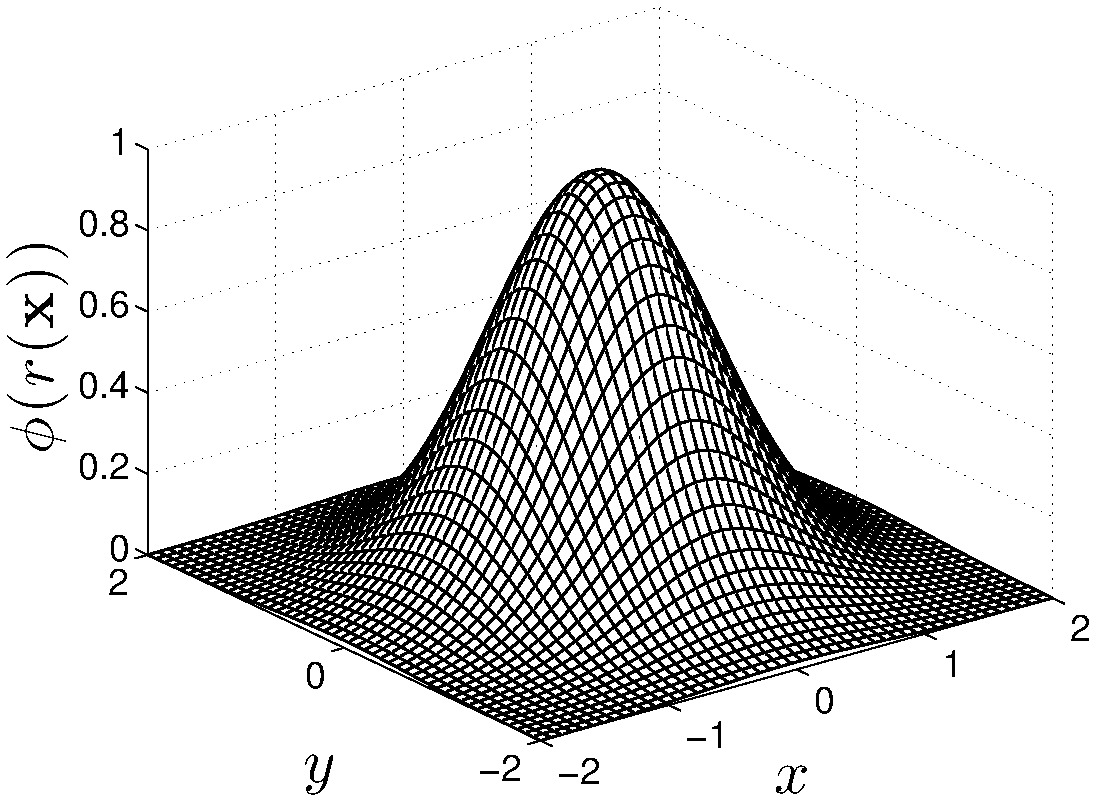
\includegraphics[width=1.0\textwidth]{../figures/paper1/figures/ga_rbf2d-eps-converted-to.pdf} 
		\caption{Gaussian}
	\end{subfigure}
	\begin{subfigure}[b]{0.25\textwidth}
	\centering
		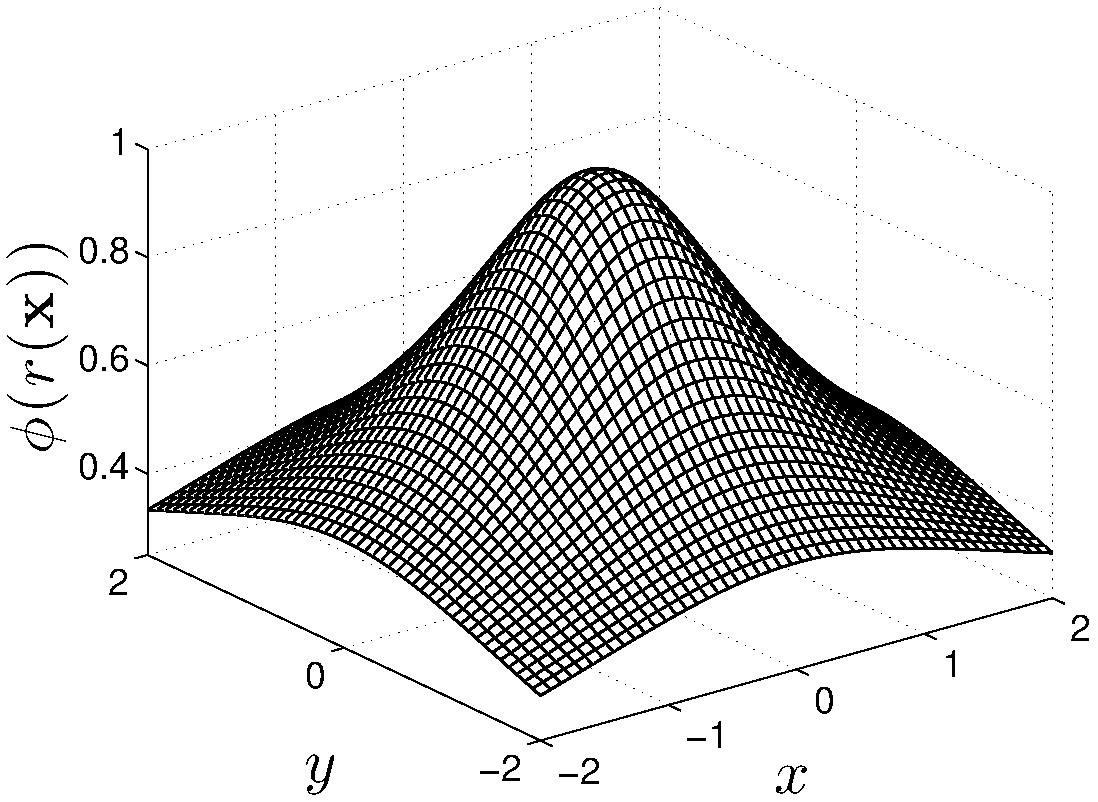
\includegraphics[width=1.0\textwidth]{../figures/paper1/figures/imq_rbf2d-eps-converted-to.pdf}
		\caption{Inverse Multiquadric}
	\end{subfigure}
	\begin{subfigure}[b]{0.25\textwidth}
	\centering
		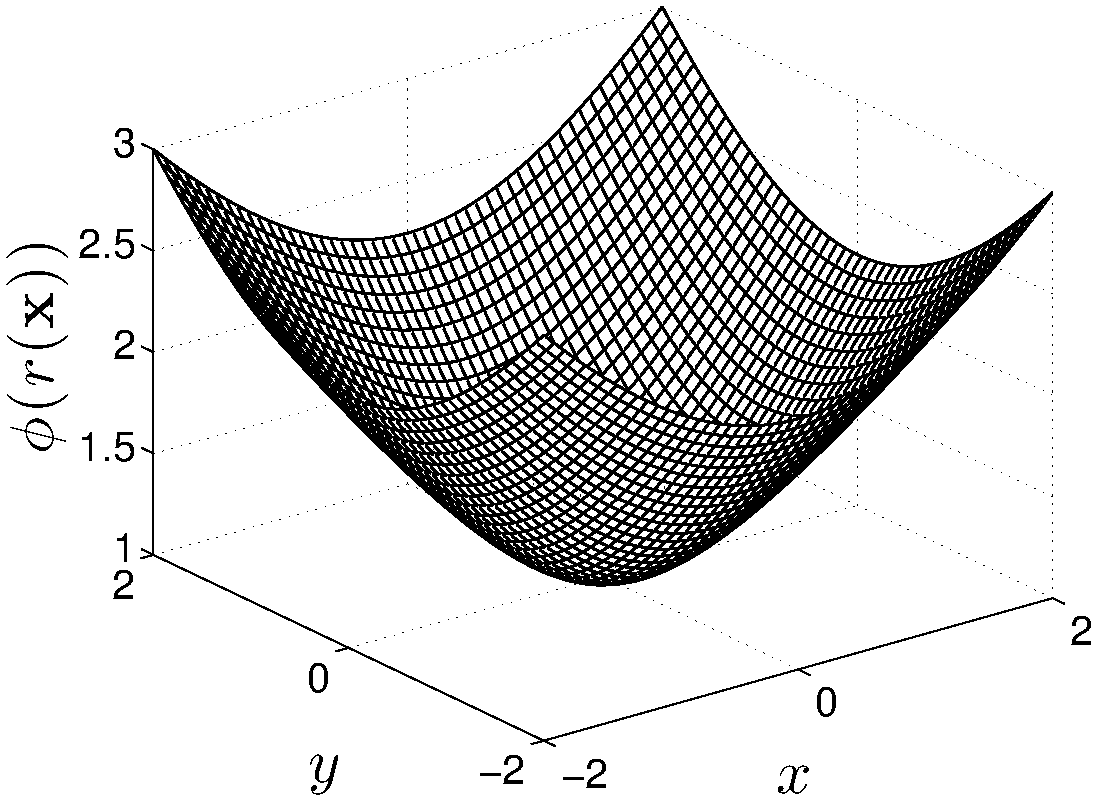
\includegraphics[width=1.0\textwidth]{../figures/paper1/figures/mq_rbf2d-eps-converted-to.pdf} 
		\caption{Multiquadric}
	\end{subfigure} 
    \caption{Commonly Used Radial Basis Functions (RBFs).}
    \label{fig:rbfs}
\end{figure}

At the core of all RBF-based PDE methods lies the fundamental problem of approximation/interpolation. Some methods (e.g., global- and compact-RBF methods) apply RBFs to approximate derivatives directly. Others (e.g., RBF-FD) leverage the basis functions to compute stencil weights, which in turn are used in generalized finite-difference approximations of derivatives. 

As ``meshless" methods, RBF methods excel at solving problems that require geometric flexibility with scattered node layouts in $d$-dimensional space. They naturally extend into higher dimensions with minimal increase in programming complexity \cite{FlyerWright07,WrightFlyerYuen10}. In addition to competitive accuracy and convergence compared with other state-of-the-art methods \cite{FlyerWright07, FlyerWright09, FlyerLehto10, WrightFlyerYuen10, FlyerFornberg11}, RBF methods boast stability for large time steps. Not all RBF methods are truly meshless. Most of them operate the same given an input set of nodes, whether or not the input includes an underlying mesh. However, some methods connect all nodes to all others (to be meshless), while methods like RBF-FD rely on stencils to connect points within small neighborhoods of one another. The generated stencils limit the scope of influence for nodes and complexity of the method, but also simulate a mesh. 

%Most literature surrounding RBF solutions for PDEs apply the concept of collocation (see Chapter~\ref{chap:background}). Recent trends in the community appear to have shifted, and RBF-FD seems to be top of the list. 


%RBF-FD is a hybrid of RBF scattered data interpolation and classical Finite Difference (FD). It shares many of the benefits from other RBF methods, like functionality on scattered node layouts in any dimension and high-order accurate solutions. Likewise, benefits akin to classical FD such as compact stencils for derivative approximation, and low computational complexity.

%Classical FD derivatives are expressed at a single node (center) as a weighted combination/difference of solution values from a small neighborhood (i.e., a stencil) around the center. Common approximations such as upwind differencing, center differencing, and other higher order approximations are of this form. 
%In similar fashion, RBF-FD combines solutions values based on stencils, but it does so in a more generalized sense than standard FD. For example, classical FD is typically restricted to regular meshes and often symmetric stencils in practice with the same set of weights for each stencil. Weights can be derived from polynomial expansion and obtained in 1D by solving a Vandermonde interpolation matrix \cite{FornbergLehto11}. Higher dimension FD stencils are composed from combinations of 1D formulas applied to each dimension. This implies restrictions on the shape/layout of stencils. In contrast to this, RBF-FD is designed for stencils with irregular node placement and can easily provide a unique set of weights for each stencil with no restrictions on stencil shape. 

%TODO:  \cite{Wright2004, Wright2003, WrightFornberg06, Chandhini2007}. 
To track the history of RBF methods, one must rewind to 1971 and R.L. Hardy's seminal research on interpolation with multi-quadric basis functions \cite{Hardy1971}. The transition from interpolation to RBF PDE methods dates back to 1990 \cite{Kansa1990a,Kansa1990b}. 
The RBF-FD method was first introduced in concept in 2000 \cite{Tolstykh2000}, but it took another few years for the method to really get a start (\cite{Shu2003}, \cite{Tolstykh2003a}, \cite{Wright2003} and \cite{Cecil2004}). Now a little over a decade old, the method is finally showing signs that it has the critical-mass following necessary for use in large-scale scientific models. At the onset of this work, most of the literature considered RBF-FD for problem sizes up to a few thousand nodes; at most into tens of thousands of nodes. Similar to most RBF methods, RBF-FD is predominantly implemented within small-scale, serial computing environments. The RBF community at-large continues to depend on MATLAB for investigation and extension development.

The goal of this dissertation is to scale RBF-FD solutions on high resolution meshes across high performance clusters, and to lead the way for its adoption within HPC and supercomputing circles. As part of this push to HPC, leveraging \emph{Graphics Processing Units (GPUs)} for computation is considered critical. GPUs, introduced in Chapter~\ref{chap:gpu_rbffd}, are many-core accelerators capable of general purpose, embarrassingly parallel computations. Accelerators represent the latest trend in HPC, where compute nodes are commonly supplemented by one or more accessory boards for offloading compute intensive tasks. Our effort leads the way for RBF-FD applicationss in an age when compute nodes with attached accelerator boards are considered key to breaching the exa-scale computing barrier \cite{GPUandExascale2011}. 

Parallelization of RBF-FD is achieved at two levels. On the first level, the
physical domain of the problem is partitioned
into overlapping subdomains, each handled by different MPI processes. All processes
operate independently to compute/load RBF-FD stencil weights, run diagnostic
tests and perform other initialization tasks. A process only computes weights
corresponding to stencils centered in the interior of its partition. After
initialization, processes work together to concurrently solve the PDE. Communication
barriers ensure that processes execute in lockstep and maintain consistent
solution values across the domain.  

The second level of
parallelization offloads tasks to the GPU at each iteration of the PDE solver. The bulk of computation in RBF-FD relies on a \emph{Sparse Matrix-Vector multiply (SpMV)} to evaluate derivatives. When mapped to the GPU, the SpMV operation is broken into two parts in order to overlap communication and computation, and amortize the cost of data transfer across multiple levels of hardware (see Chapter~\ref{chap:multigpu_rbffd}). 
% Although the stencil weight calculation is also data-parallel, we assume that in this context that the weights are precomputed and loaded once from disk during the initialization phase. 

%Additional key challenges lie in the choice of grid, the choice of stencil, and stability of scalable solutions. 
%To demonstrate Chapter~\ref{chap:applied_rbffd} verifies 


%
%Even today, RBFs are still up-and-coming in the scientific world with many avenues of research left to consider. Global formulations are understood to have spectral convergence properties, high accuracy and other benefits like adaptivity and ease of implementation over meshed methods \cite{Fasshauer:2007}. However, little is known about the behavior of local and RBF-FD methods. Open questions include (but are in no way limited to): a) ideal node placement to eliminate singularities; b) data-structures for stencil storage and evaluation; c) problem sizes larger than a few thousand nodes; and d) parallel implementations across new heterogeneous multi- and many-core architectures. In response to this, our group, in collaboration with researchers assembled from a national lab and four universities (see Chapter~\ref{chap:funding}), has been granted funds by the National Science Foundation to collaboratively:
%
%\begin{quote}
%\emph{``Bring RBFs to the forefront of multi-scale geophysical modeling by developing fast, efficient, and parallelizable RBF algorithms in arbitrary geometries, with performance enhanced by hardware accelerators, such as graphic processing units (GPUs)."} \cite{RBF_proposal:2009}
%\end{quote}
%
%



The layout of this document is as follows. This chapter continues with a survey of work related to parallelizing RBF-FD, targeting the GPU, and spanning a multi-GPU cluster. Chapter~\ref{chap:background} provides a historical survey of RBF methods as a backdrop to present RBF-FD in Chapter~\ref{chap:rbffd_method}. Chapter~\ref{chap:stencils} introduces a new algorithm for generating RBF-FD stencils as a faster alternative to the RBF community favorite, $k$-D Tree. In Chapter~\ref{chap:distributed_rbffd}, the first scalable implementation of RBF-FD to span one thousand processors is described in detail. Chapter~\ref{chap:gpu_rbffd} continues with the challenge of offloading computation to GPUs, and Chapter~\ref{chap:multigpu_rbffd} expands the discussion to RBF-FD on a multi-GPU cluster. In Chapter~\ref{chap:applications} the parallel RBF-FD implementation is applied and verified on the solutions of both explicit and implicit geophysical PDEs. Finally, Chapter~\ref{chap:conclusions} concludes with a summary of novel contributions, results and a discussion on future directions.

\section{On Parallel/Distributed RBF-FD} 

%TODO: why implement independent of PETSc, Deal.II, Trilinos, etc. 

%\authnote{Related work for start of Parallel/GPU chapter}
Parallel implementations of RBF methods rely on \emph{domain decomposition}. Depending on the implementation, domain decomposition not only accelerates solution procedures, but can decrease the ill-conditioning that plague all global RBF methods (\cite{Divo2007}). The ill-conditioning is reduced if each domain is treated as a separate RBF domain, and the boundary update is treated separately. Domain decomposition methods for RBFs were introduced by Beatson et al. \cite{Beatson2000}. Their work provided a solution to solve problem sizes into the millions of nodes.

This work leverages a domain decomposition, but not for the purpose of conditioning. Instead subdomains are distributed across multiple compute nodes and scaling RBF-FD across more than a thousand CPU cores of an HPC cluster. Add to this a twist to incorporate a novel implementation on the GPU with overlapping communication and computation. This combination is unmatched in related work. However, RBF methods do have a bit of history of parallel implementations. 

In 2007, Divo and Kassab \cite{Divo2007} used a domain decomposition method with artificial 
subdomain boundaries for their implementation of a local collocation method \cite{Divo2007}. 
The subdomains are processed independently, with derivative values 
at artificial boundary points averaged to maintain global consistency of physical values. Their implementation 
was designed for a 36 node cluster, but benchmarks and scalability tests are not provided.

% Divo: it seems almost unnecessary to use domain decomposition if they have the local method.
% I suppose the domain decomposition is necessary for averaging physical values more than RBF collocation.
However, research on the parallelization of RBF algorithms to solve PDEs on multiple CPU/GPU architectures is essentially non-existent. We have found three studies that have addressed this topic, none of which implement RBF-FD but rather take the avenue of domain decomposition for global RBFs (similar to a spectral element approach). In \cite{Divo2007}, Divo and Kassab introduce subdomains with artificial boundaries that are processed independently. Their implementation was designed for a 36 node cluster, but benchmarks and scalability tests are not provided. Kosec and \v{S}arler \cite{Kosec2008} parallelize coupled heat transfer and fluid flow models using OpenMP on a single workstation with one dual-core processor. They achieved a speedup factor of 1.85x over serial execution, although there were
no results from scaling tests. Yokota, Barba and Knepley \cite{Yokota2010} apply a restrictive additive Schwarz domain decomposition to parallelize global RBF interpolation of more then 50 million nodes on 1024 CPU processors.

Kosec and \v{S}arler \cite{Kosec2008} have the only known (to our knowledge) OpenMP implementation for RBFs. The authors parallelize coupled heat transfer 
and fluid flow problems on a single workstation. 
The application involves the local RBF collocation method, explicit time-stepping and Neumann boundary conditions. A speedup 
factor of 1.85x over serial execution was achieved by executing on two CPU cores; no further 
results from scaling tests were provided. 

Stevens et al. \cite{Stevens2009a} mention a parallel implementation under development, but no document is available at this time. 

Perhaps the most competitive parallel implementation of RBFs is the PetRBF branch of PETSc \cite{Yokota2010}. The authors of PetRBF have implemented a highly scalable, efficient RBF interpolation method based on compact RBFs (i.e., they operate on sparse matrices). The authors demonstrate efficient weak scaling of PetRBF across 1024 processes on a Blue Gene/L, and strong scaling up to 128 processes on the same hardware. On the Blue Gene/L, PetRBF is demonstrated to achieve an impressive 74\% parallel weak scaling efficiency on 1024 processes (operating on over 50 million points), and 84\% strong scaling efficiency for 128 processes. Strong scaling was also tested on a Cray XT4, where strong scaling tops out at 36\% for 128 processes, a respectable number---and similar to observed results for our own code on for the same number of processes (see Chapter~\ref{chap:distributed_rbffd}).  


%Within the scope of this paper we detail our method for spanning RBF-FD across multiple CPU/GPU processors and emphasize numerical validation of the implementation rather than optimization strategies. We will consider optimization in future work. The calculations are performed on Keeneland, a high performance computing installation supported by the National Science Foundation and located at Oak Ridge National Lab. Keeneland currently has 240 CPUs accompanied by 360 NVidia Fermi class GPUs with at least double that number expected by the end of 2012 \cite{Vetter2011}.



\section{On GPU RBF Methods (Incomplete)}

With regard to the latter, there is some research on leveraging RBFs on GPUs in the fields of visualization \cite{Cuntz2007,Weiler2005},  surface reconstruction \cite{Corrigan2005,Carr2003}, and neural networks \cite{Brandstetter2008}.

 %Originally GPUs were designed as parallel rasterizing units. They had limited logic control in contrast to the serial CPUs and their advanced branching and looping logic. 
%
%Gradually new and complex logic was added to the GPU to produce the shader languages that allowed developers to customize specific parts of the rendering pipeline. This allowed scientific problems such as the diffusion equation to be solved in process of rendering \cite{Harris2005}. In other words, the GPU was tricked into computing.
%
%The year 2006 brought the modern age of GPU computing with the introduction of CUDA from NVidia. The high level language allowed scientists to leverage the GPU as a parallel accelerator without all of the overhead of setting up graphics contexts and tricking the hardware into computing. Memory management is still the developer's responsibility, but compiler transforms generic C/Fortran code to GPU instruction set. 
%
%Scientific Computing has seen a widespread adoption of GPGPU because of the goal to get to ``exa-scale'' computing, which may only be possible in the near future with the help of GPU accelerators \cite{GPUandExascale2011}. 
%
%NVidia is not the only company involved in many core parallel accelerators. Other groups like AMD and Intel have been increasing the number of cores as well. The end effect is a hybridization where CPUs look similar to GPUs and vice-versa. 
%
%Until 2009, the hardware distinction required that developers target parallelism on CPUs and GPUs using different languages. Then the OpenCL standard was drafted and implemented. OpenCL is a parallel language that strives to provide functional portability rather than performance. 
%
%We focus on the OpenCL language within this dissertation with confidence that hardware will change frequently. In fact, every 18 months \cite{CudaGuide2011} shows a new release of GPU hardware, many-core CPU hardware and extensions to parallel languages. But if hardware is constantly changing, then one must focus on a high level implementation that allows portability across hardware. Enter the Open Compute Language (OpenCL) in 2009. OpenCL is standards based a to carry our implementations into the future regardless of what hardware and which company survive. 


Related work on RBFs and GPUs is sparse. In 2009, Schmidt et al. \cite{Schmidt2009a, Schmidt2009b} implemented a global RBF method for Tsunami simulation on the GPU using the AccelerEyes Jacket \cite{JacketGuide2009} add-on for MATLAB. Jacket provides a MATLAB interface to data structures and routines that internally call to the NVidia CUDA API. Their model was based on a single large dense matrix solve, and with the help of Jacket the authors were able to achieve approximately 7x speedup over the standard MATLAB solution on the then current generation of the MacBook Pro laptop. The authors compared the laptop CPU (processor details not specified) to the built-in NVidia GeForce 8600M GT GPU. Schmidt et al.'s implementation was the first contribution to the RBF community to leverage accelerators. The results were significant and promising, but no further contributions were made on the topic. 

While both Schmidt et al.'s method and the method presented here are based on RBFs, the two problems are only distantly related when it comes to implementation on the GPU. Dense matrix operations have a high computational complexity, are considered ideal (or near to) by linear algebra libraries like BLAS \cite{BLAS} and LAPACK \cite{Lapack1999}, and were demonstrated to fit well on GPUs from the onset of General Purpose GPU (GPGPU) Computing. In fact, NVidia included CUBLAS \cite{CudaToolkitDoc} (a GPU based BLAS library for their hardware) with their initial public release of the game-changing CUDA development kit in 2006. In stark contrast to this, sparse matrix operations have minimal computational complexity and are less than ideal for the GPU.


Earlier this year (2013), Cuomo et al. \cite{Cuomo2013} implemented RBF-interpolation on the GPU for surface reconstruction. Their implementation utilizes PetRBF \cite{Yokota2010}, and new built-in extensions that allow GPU access within PETSc. PETSc internally wraps the CUSP project \cite{Cusp2012} for sparse matrix algebra on the GPU. With the help of these libraries, Cuomo et al. solve and apply sparse interpolation systems on the GPU for up to three million nodes on an NVidia Fermi C1060 GPU (4GB). They compare results to a single core CPU implementation on an Intel i7-940 CPU and demonstrate that the GPU accelerate their solutions between 6x and 25x. Unfortunately, the authors do not show evidence of scaling the interpolation across multiple GPUs; so while evidence exists that PetRBF now has full GPU support, it remains to be seen how well the code can scale in GPU mode. 
 
\section{On Multi-GPU Methods}
 
Multi-GPU Jacobi iteration for Navier stokes flow in cavity \url{http://scholarworks.boisestate.edu/cgi/viewcontent.cgi?article=1003&context=mecheng_facpubs}

Thibault et al. have multiple works on Multi-GPU and overlapping comm and comp. 

The latest version of PETSc includes GPU support. PETSc is a widely-used library for distributed sparse and dense matrix algebra. 

\section{Major Contributions}

Within this thesis readers should expect to find the following major contributions to the communities surrounding RBF methods, GPGPU, and HPC: 
\begin{itemize} 
\item The first implementation of RBF-FD on GPUs, with one and many GPU environments considered. 
\begin{itemize} 
\item Multiple GPU kernels are tested, including custom OpenCL kernels for RK4 time-stepping and 
\end{itemize} 
\item The first implementation of RBF-FD on multiple CPUs through the use of domain decomposition
\item The first application of the Fixed-Grid neighbor query algorithm to generate stencils for RBF-FD. 
\end{itemize}



\ifstandalone
%Bei direkter Übersetzung sollte gleich noch das Literaturverzeichnis rein.
\bibliographystyle{plain}
\bibliography{merged_references}
\end{document}
\else
\expandafter\endinput
\fi
 
%\chapter{Grid Generation}

Topics: 
\begin{itemize} 
    \item Neighbor queries with LSH and k-D Tree
    \item Node ordering
    \item Impact on Conditioning
    \item Impact on Convergence (Move to GMRES chapter)
    \begin{itemize} 
        \item CVT based load-balancing for minimum communication and equal computation
        \item LSH order inside partitions and before CVT 
    \end{itemize}
    \item Domain Decomposition
\end{itemize} 

%\chapter{Parabolic Equations}

Topics to cover
\begin{itemize} 
    \item PDE form
    \item Test cases: heat
    \begin{itemize} 
        \item TODO: todo test cases sauron, annulus and nested sphere, ellipsoid and Macaque (gen CVT inside macaque) 
    \end{itemize}
\end{itemize}

%\chapter{Hyperbolic Equations}

Topics to cover
\begin{itemize} 
    \item Explicit solve for hyperbolic equation
    \item Decomposition
    \item Test cases (vortex, cosine)
    \item performance increase
    \item Optimizations
    \begin{itemize} 
        \item Todo: finish optimizations (overlap comm, improve kernels) 
    \end{itemize} 
\end{itemize}

%\chapter{Multi-GPU Preconditioned GMRES}


\section{Introduction}
This handout follows the implementation of my Parallel (Multi-GPU) GMRES algorithm. 

\section{TOREAD} 

http://www.irisa.fr/sage/recherche/sparsesolver.html

(consider Deflated GMRES for gpu. Doesnt appear to have been tested. Li and Saad point out that Deflated PCG was tested with success.)

\section{Related Work: Li and Saad 2011} 

Li and Saad demonstrated that for unstructured matrices SpMV kernels can be up to 10x faster than the CPU (Tesla C1060 vs Intel Xeon E5504). 
Their Incomplete Cholesky (special case of ILU) and Conjugate Gradient method on the GPU is up to 3x faster. 
An ILU preconditioned GMRES method can be up to 4x faster. 

\authnote{ THIS IS MY GOAL: at least 4x speedup for my ILU0 and GMRES for RBF-FD unstructured matrices} 

\section{Related Work: Bahi et al. 2011}
A multi-GPU implementation of GMRES was introduced in 2011 by Bahi, et al. \cite{Bahi2011}. In Algorithm~\ref{alg:gmres}, I have included the original pseudocode presented in \cite{Bahi2011} and {\color{blue}comments} for a discussion of what the algorithm does. 

\begin{algorithm}                      % enter the algorithm environment
\caption{Left-preconditioned GMRES with restarts}          % give the algorithm a caption
\label{alg:gmres}                           % and a label for \ref{} commands later in the document
\begin{algorithmic}[1]                    % enter the algorithmic environment
    \State $\varepsilon$ (tolerance for the residual norm $r$), $x_0$ (initial guess), and set $convergence = false$
    \While{ $convergence == false$}
    \State $r_0 = M^{-1} (b-Ax_0)$ \Comment{{\color{blue} They left off details of restarts, is the rest of their algorithm accurate?}}
    \State $\beta = ||r_0||_2$
    \State $v_1 = r_0 / \beta$ \Comment{ {\color{blue}This should really read: $v_1 = \frac{1}{\beta} r_0$)}}
	\For {$j=1$ to $m$} \label{alg:gmres_rotation_loop_start} \Comment{ {\color{blue}$m$ is the $restart$ input parameter ($\#$ of iters between restarts) } }
			\State $w_j = M^{-1} A v_j$
			\For {$i = 1$ to $j$}\label{alg:gmres_inner_loop_start}\Comment{{\color{blue}Key: we do $j$ iterations so the amount of work always grows }}  
				\State $h_{i,j} = (w_j, v_i)$ \Comment{{\color{blue}$(\cdot,\cdot)$ is an inner/dot product (usually $< \cdot, \cdot >$) }}
				\State $w_j = w_j - h_{i,j} v_i$
			\EndFor \label{alg:gmres_inner_loop_stop}
			\State $h_{j+1, j}  = ||w_j||_2$			\Comment{ {\color{blue}This $(m+1)\times m$ upper Hessenberg matrix must be stored }}
			\State $v_{j+1} = w_j / h_{j+1,j}$		\Comment{{\color{blue}This forms an orthonormal basis $V_m$ and must be stored ($N \times m$ matrix)}}
	\EndFor\label{alg:gmres_rotation_loop_stop} 
	\State Set $V_m = [v_1, \cdots, v_m]$ and $\bar{H}_m = (h_{i,j})$ an upper Hesssenberg matrix of order $(m+1)\times m$
	\State \label{alg:gmres_least_squares} Solve a least-square problem of size $m$: $\min_{y \in \R^m} ||\beta e_1 - \bar{H}_m y||_2$	\Comment{{\color{blue}Ambiguous. Will clarify.}}
	\State $x_m = x_0 + V_m y_m$ \label{alg:gmres_residual_norm}
	\If { $||M^{-1}(b-Ax_m)||_2  < \varepsilon$ }
		\State $convergence = true$
	\EndIf
	\State $x_0 = x_m$
    \EndWhile
\end{algorithmic}
\end{algorithm}

\subsection{Communication Points} 

In \cite{Bahi2011} the authors point out that communication happens at two types of points in the algorithm: \begin{enumerate} \item Before SpMV operations, and \item After vector operations \end{enumerate}. I have added markup to their pseudo-code in Algorithm~\ref{alg:gmres_comm} to illustrate where they perform communication. 

\begin{algorithm}                      % enter the algorithm environment
\caption{Left-preconditioned GMRES with restarts and {\color{red} communication poins} }          % give the algorithm a caption
\label{alg:gmres_comm}                           % and a label for \ref{} commands later in the document
\begin{algorithmic}[1]                   % enter the algorithmic environment
    \State $\varepsilon$ (tolerance for the residual norm $r$), $x_0$ (initial guess), and set $convergence = false$
    \While{ $convergence == false$}
    \State {{\color{red} MPI\_AlltoAllv() }}
    \State $r_0 = M^{-1} (b-Ax_0)$ 	
    \State $\beta = ||r_0||_2$		
	\State{{\color{red} MPI\_Allreduce() }}	 	
    \State $v_1 = r_0 / \beta$
	\For {$j=1$ to $m$} 
			\State {{\color{red} MPI\_AlltoAllv() }}
			\State $w_j = M^{-1} A v_j$			 	
			\For {$i = 1$ to $j$}
				\State $h_{i,j} = (w_j, v_i)$ 				
				\State{{\color{red} MPI\_Allreduce() }}
				\State $w_j = w_j - h_{i,j} v_i$
			\EndFor 
			\State $h_{j+1, j}  = ||w_j||_2$			
			\State{{\color{red} MPI\_Allreduce() }}
			\State $v_{j+1} = w_j / h_{j+1,j}$	
	\EndFor
	\State Set $V_m = [v_1, \cdots, v_m]$ and $\bar{H}_m = (h_{i,j})$ an upper Hesssenberg matrix of order $(m+1)\times m$
	\State Solve a least-square problem of size $m$: $\min_{y \in \R^m} ||\beta e_1 - \bar{H}_m y||_2$
	\State $x_m = x_0 + V_m y_m$
	\If { $||M^{-1}(b-Ax_m)||_2 < \varepsilon$ }
		\State $convergence = true$
	\EndIf
	\State{{\color{red} MPI\_Allreduce() }}
	\State $x_0 = x_m$
    \EndWhile
\end{algorithmic}
\end{algorithm}

\subsection{Practical Implementations}

In Algorithm~\ref{alg:gmres}, line~\ref{alg:gmres_least_squares} ambiguously states we need to solve a least-squares problem. 

%This ambiguity is also present in Saad's book (see e.g., page 165, \cite{Saad2003}) although the authors return on page 169 to discuss Givens rotations and other useful details for ``Practical Implementation". This section summarizes a few of those details. 

We could take the algorithm as is and express the least-squares problem as 
\begin{equation} 
\bar{H}_m^T \beta e_1 - \bar{H}_m^T \bar{H}_m y = 0 \label{eq:least_squares}
\end{equation}
for a cost of O($m^3$) operations on line~\ref{alg:gmres_least_squares}. If $m$ is small this is not a concern. However, it is common practice instead to find the implicit QR decomposition of $\bar{H}_m$ to reduce the complexity to O($m^2$). 

Saad and Schultz \cite{Saad1986} detail an efficient method of computing plane rotations at the end of each inner-loop iteration (i.e., just before line~\ref{alg:gmres_rotation_loop_stop} of Algorithm~\ref{alg:gmres}). Their method computes one Givens rotation at a cost of O($m$) per iteration, such that at the end of the loop, the QR factorization is implicitly formed with an overhead of O($m^2$). With the QR factor, the minimization problem transforms to 
$$\min_{y \in \R^m} ||Q^T (\beta e_1 - \bar{H}_m y) ||_2 = \min_{y \in \R^m} ||g_m - R_m y||_2$$
where $R_m$ is the upper triangular $m\times m$ factor of $\bar{H}_m$ from the QR process, and $g_m = Q^T \beta e_1$ has been updated at each iteration. Now, using the knowledge that the 2-norm of a vector is invariant under orthogonal transformations (i.e., the matrix $Q^T$), our minimization problem reduces to solving $$ R_m y = g_m $$ which can be done with a simple upper triangular back solve. 

Saad and Schultz \cite{Saad1986} also demonstrate that by using the implicit QR factorization, the residual norm of the approximate solution $x_m$ is available at every iteration without explicitly forming $x_m$ on Line~\ref{alg:gmres_residual_norm}. Instead, due to the Givens rotations of system, the residual norm is always available in the $(k+1)$-st component of $g_k$. The explicit formation of $x_m$ involves the product of $N \times m$ matrix $V_m$ and $N$ length vector $x_m$. Therefore, using the implicit residual norm and postponing the formation of our solution saves a significant O($Nm$) operations per iteration. 

As the first multi-GPU GMRES paper, Bahi et al. \cite{Bahi2011} do not specify if they use Givens rotations for efficiency. The description of their algorithm states one thread on the GPU takes responsibility in Algorithm~\ref{alg:gmres} at line~\ref{alg:gmres_least_squares} and solves the size-$m$ least squares problem. This leads me to believe they solve Equation~\ref{eq:least_squares}. They also mention a kernel that forms a local view of $x_m$ on line~\ref{alg:gmres_residual_norm}, which further argues against soliciting the help of the implicit QR. \authnote{THIS COULD BE A NEW CONTRIBUTION. Do the plane rotations require additional synchronization? Do the plane rotations impact convergence? Is there a reason to avoid plane rotations stated in other parallel GMRES algorithms publications?} 


\section{Related Work: Dekker 2000}
In 2000, Dekker \cite{Dekker2000} published a report describing the Parallel GMRES method. His approach was to apply an additive schwarz decomposition to the standard GMRES (with Givens rotations) and then add a few tweaks to increase scalability. The punch line of his method is that it increases computational overhead per processor in order to reduce the overall communication time. This is ideal for GPUs where the cost of communication includes both CPU-CPU and two way CPU-GPU transfers. I suspect this is the approach we want to take. However, in Dekker's subsequent papers (see \cite{Dekker2001}, \cite{Dekker2005}) he mentions a requirement for his convergence studies to have red-black ordering on the nodes. This is not possible with RBF-FD as far as I know. Red-black ordering would require us to partition every other node into red and the rest in black. This can be extended to more than two colors, but I'm not sure our connectivity would allow for the separation in matrix blocks that he leverages in the latter papers. \cite{Dekker2000} does not appear to have this requirement but I need more exposure with the method to be certain.  


\section{CUSP Implementation} 

To implement my own multi-GPU Parallel GMRES, I chose to leverage the existing code-base of libraries like ViennaCL and CUSP. Starting with our existing physical domain partitioning, we can drop in our calls to ``sendrecvUpdates(...)" for the MPI\_AlltoAll calls. Then we just need to add an MPI\_Allreduce replacement, and we should be nearly finished. 

The one aspect of this parallel implementation that I'm concerned with is the least-squares solution. In CUSP and ViennaCL, the implicit rotations are used to accelerate the least squares step. If this cannot span multiple GPUs---so far the discussion is that its high in communication cost, but nothing saying its impossible---then I will have to re-work more of their algorithms. 

I'll start by 

 


%\appendix
%\chapter{TODO}
%\input todolist

% The BibTeX bibliography/references section.  View the file
% 'myrefs.bib' to get a feel for what these entries may look like.
% By using the optional \nocite{*} line, every entry in 'myrefs.bib'
% will be inserted into the bibliography.  Otherwise, only entries
% that have been cited with \cite{key} somewhere in the text will
% be included.
%\nocite{*}
% Or individually reference papers you want to include without citation: 
%\nocite{Vuduc2005}

%\bibliographystyle{plain}
%\bibliography{references}

%\begin{biosketch}
This is my biography.
\end{biosketch}


\end{document}
